% !TeX program = pdflatex
\documentclass{iutbscthesis}

%% --- Line breaking --------------------------------------------------------
% Long ODC type names and code identifiers leave few break points. Give TeX a
% final pass with extra stretch rather than letting lines run into the margin.
\setlength{\emergencystretch}{3em}

%% --- Long literals that must be allowed to break across lines --------------
\newcommand{\modelname}{\texttt{gemini-\allowbreak 3.1-\allowbreak flash-\allowbreak lite-\allowbreak preview}}

%% --- Diagrams (TikZ figures in Chapters 2 and 4) ---------------------------
\usepackage{tikz}
\usetikzlibrary{arrows.meta,positioning,calc,shapes.geometric,fit,backgrounds}

\addbibresource{citations.bib}

% Title
\title{Orthogonal Defect Classification on Defects4J Using an LLM-Driven Scientific Approach}

% Authors
\addauthor{Md. Sakib Hossain}{210042133}
\addauthor{Mohammad Nahiyan Kabir}{210042168}
\addauthor{Hasin Mahtab Alvee}{210042174}

% Supervisor
\supervisor{Lutfun Nahar Lota}{Assistant Professor}{Department of Computer Science and Engineering}

% Co-supervisor
\addcosupervisor{Ishmam Tashdeed}{Lecturer}{Department of Computer Science and Engineering}

% Department
\department{Department of Computer Science and Engineering}

% Program
\program{BACHELOR OF SCIENCE IN COMPUTER SCIENCE AND ENGINEERING}

% Book submission date
\defensedate{17}{September}{2026}

\begin{document}

%-------------------------- FRONT MATTER --------------------------%

\coverpage
\pagenumbering{roman}
\titlepage
\declarationofcandidate

\dedicatedto{our families, friends, and mentors}

\tableofcontents
\listoffigures
\listoftables

\clearpage

\begin{abbreviations}
    \abbr{APR}{Automated Program Repair}
    \abbr{API}{Application Programming Interface}
    \abbr{CFG}{Control Flow Graph}
    \abbr{CI}{Confidence Interval}
    \abbr{CLI}{Command Line Interface}
    \abbr{CoT}{Chain-of-Thought}
    \abbr{D4J}{Defects4J}
    \abbr{DFG}{Data Flow Graph}
    \abbr{LLM}{Large Language Model}
    \abbr{ML}{Machine Learning}
    \abbr{NLP}{Natural Language Processing}
    \abbr{ODC}{Orthogonal Defect Classification}
    \abbr{RQ}{Research Question}
    \abbr{SDLC}{Software Development Life Cycle}
    \abbr{SVM}{Support Vector Machine}
    \abbr{TVD}{Total Variation Distance}
\end{abbreviations}

\begin{acknowledgement}
We would like to express our sincere gratitude to our supervisor, Lutfun Nahar Lota, and our co-supervisor, Ishmam Tashdeed, for their continuous guidance and support throughout this research. Their expertise and encouragement helped shape this work from concept to completion.

We are also grateful to the Network and Data Analysis Group (NDAG) Lab at IUT for providing the research environment and resources that made this thesis possible.

Finally, we thank the maintainers of the Defects4J benchmark, whose careful curation of reproducible real-world bugs made this study possible at all.
\end{acknowledgement}

\begin{abstract}
Defect classification turns isolated bug reports into process-level signals that guide debugging strategy and quality improvement. Defects4J is the standard benchmark for empirical Java fault studies, yet no prior work has labelled it with a principled, semantic, root-cause taxonomy. Existing efforts cover only tens to a few hundred bugs, use structural or patch-shape taxonomies that describe \emph{how} a bug manifests rather than \emph{why} it exists, or depend on post-fix code that is unavailable during real triage.

This thesis presents an automated pipeline that classifies Defects4J bugs into the seven Orthogonal Defect Classification (ODC) Design/Code defect types using Large Language Model reasoning. We separate \emph{what label space} the model may answer in from \emph{how} it reasons toward a label, giving a controlled space of conditions whose strongest setting is an enforced loop whereby the model must commit to a hypothesis and probe held-back evidence before it is allowed to conclude. An explicit ``Other'' escape category lets us measure the taxonomy's coverage rather than assume it. Every bug is classified twice, once from pre-fix evidence (symptoms only) and once from post-fix evidence (with the developer's actual fix), which supplies an evaluation reference for a benchmark that carries no labels.

Across 257 bugs from five projects, three ODC types account for almost the entire benchmark, and the type mix does not vary significantly across projects. The escape category was offered in every classification and never once used, bounding the true escape rate below one percent. A classification made before the fix exists reproduces the fix-aware reference on \textbf{73.5\%} of bugs (Cohen's $\kappa = 0.577$), close to the ceiling we measure for two fix-aware runs of the same model. The enforced loop significantly improves chance-corrected agreement over a strong few-shot prompt and halves the spread of reliability across projects, with its largest gains where the single-shot prompt is weakest. About a quarter of labels change once the fix becomes visible, but three quarters of those changes stay inside the same three mutually ambiguous types, and the aggregate type distribution barely moves, which is the level ODC was designed to operate at.
\end{abstract}

%-------------------------- MAIN BODY --------------------------%
\pagenumbering{arabic}

% ================================================================
% CHAPTER 1: INTRODUCTION
% ================================================================
\chapter{Introduction}

Software bugs are an unavoidable part of the development process. Even carefully written programs contain defects that cause unexpected behaviour, crashes, or incorrect results. Finding a bug is only the first step. Understanding \emph{what kind} of bug it is, \emph{why} it happened, and \emph{how} it should be fixed is equally important for improving software quality over time \cite{catolino2019not}.

Put more directly: software bugs are unavoidable, but how much they cost depends on how quickly and accurately a team can classify them. Defect classification is what turns a raw bug report into that identification, because different defect types call for different debugging strategies, resource allocations, and repair approaches \cite{catolino2019not, hirsch2022using}.

In practice, developers spend a significant portion of their time triaging and debugging reported issues. Bug categorization makes this process more efficient by grouping defects into meaningful categories that guide debugging strategies and resource allocation \cite{andrade2025empirical}. Predicting a bug's category early, from its report, helps teams prioritize work before anyone opens the code \cite{hirsch2022using}. Structured categorization also provides actionable measurements that managers and developers can use to improve their processes \cite{chillarege1992odc}.

The value of that categorization compounds over time. A single labelled bug tells a developer which debugging strategy to reach for. A thousand labelled bugs tell a team something quite different: which kinds of mistake their process keeps producing, whether that profile is changing release over release, and where a review checklist or a static analysis rule would actually pay for itself. This is the use ODC was designed for, and it is a use that depends on the labels being consistent and comparable, not merely plausible. It is also the reason a taxonomy matters more than raw labelling accuracy: a set of individually sensible labels that cannot be counted together is of no process value at all, a point we quantify directly in Section~\ref{sec:rq4a}.

Manual triage still gives the best results, but it does not scale to large benchmark datasets \cite{andrade2025empirical}. To test whether classification can be automated, we need two things: a dataset large enough to be convincing, and a benchmark rich enough to classify from.

\section{Defects4J: The Benchmark Dataset}

Defects4J is a curated database of real, reproducible Java bugs paired with developer-written patches and regression test suites \cite{just2014defects4j}. It has grown to include over 830 active bugs across 17 Java projects and serves as the standard benchmark for empirical software engineering research, including fault localization, automated program repair, and testing studies \cite{rafi2024revisiting, durieux2018automatic}.

Defects4J is exactly that benchmark, the one most empirical Java fault studies already build on. It gives us a large, curated set of reproducible bugs across 17 open-source projects, and every bug comes with a rich bundle of evidence: the original bug report, the tests that trigger it, the buggy and fixed source, and the buggy-to-fixed diff. That richness is exactly what makes Defects4J such a good fit for automated classification research.

These artifacts suit automated analysis because they give several \emph{independent} perspectives on the same defect. A stack trace says where the program failed. A bug report says what the user noticed. A failing test says what behaviour was expected. A diff says what the developer eventually changed. Each is a partial view, and each is partial in a different way, so a classifier that can read several at once has far more to work with than one reading any single source. This is also precisely why the benchmark suits a \emph{reasoning} pipeline rather than a text classifier: the evidence is heterogeneous, and deciding which piece of it to trust is itself part of the diagnostic task.

One property of Defects4J deserves emphasis here, because the entire evaluation of this thesis rests on it. Every bug ships with the developer's actual fix. That means we can construct, for any bug, two versions of the same case file that differ in exactly one respect: whether the fix is visible. Nothing else in the evidence changes. That single controlled difference is what gives us an evaluation reference in a dataset that carries no labels, and Section~\ref{sec:eval} develops it into the four-level framework this thesis evaluates against.

\section{Motivation}

Despite the widespread use of Defects4J in software engineering research, no study has ever fully classified its bugs using a principled, root-cause taxonomy. Existing classification efforts fall into three groups, each with a different focus and a different limitation.

First, structural approaches such as the work of \textcite{vanderspuy2025anatomy} classify bugs by their control-flow and data-flow graph representations. This covers 488 bugs across seven projects, but it captures how bugs manifest \emph{syntactically} rather than why they exist \emph{semantically}. A missing null check and a completely absent feature can produce similar control-flow changes while representing fundamentally different kinds of mistake.

Second, patch-level taxonomies such as the Defects4J Dissection by \textcite{sobreira2018dissection} classify repair actions for 395 bugs from an older version of the dataset. This describes what developers changed, not the defect mechanism that made the change necessary.

Third, small-sample inspections such as the work of \textcite{jiang2019manual} manually analyse 50 randomly selected bugs. The analysis is detailed, but the authors themselves note the limited external validity of examining only 50 bugs.

And yet, despite this richness, no one has produced a full, semantic labelling of the benchmark. We looked at why, and existing classification work falls into three groups, each with a different focus: control- and data-flow analyses capture \emph{how} a bug manifests syntactically \cite{vanderspuy2025anatomy}; patch taxonomies describe \emph{what} developers changed \cite{sobreira2018dissection}; and small-scale manual inspections do not scale \cite{jiang2019manual}. None of them classifies bugs into a semantic defect-type taxonomy at the scale of the full benchmark. That gap motivates an automated, scalable classification approach that goes beyond surface-level structural patterns.

Large Language Models are a plausible way to close it. Recent work shows that code-aware LLM reasoning can classify software artifacts competitively, provided the prompt is designed carefully \cite{colavito2024llm, koyuncu2025exploring, nong2024cot}. Left unconstrained, however, LLM classification drifts: with no fixed label space, different runs assign incompatible categories to the same bug \cite{koyuncu2025exploring}, producing labels that cannot be aggregated or compared. Supplying a taxonomy, and defining its labels explicitly, measurably changes what the model predicts \cite{li2024knowbug}, and Section~\ref{sec:rq4a} quantifies how severe the unconstrained case is on our own data. A principled taxonomy fixes that by turning classification into a bounded, semantically grounded decision problem.

But a forced, fixed schema introduces the opposite failure. It manufactures false certainty for defects that genuinely do not fit any of its categories. Our answer is to treat the taxonomy's own coverage as something to \emph{measure} rather than assume: we give the model an explicit escape category, ``Other'', so a defect that falls outside the seven types becomes recorded data instead of a mislabelled forced choice.

One more constraint shapes the whole design. In this study we classify defects using \textbf{pre-fix evidence} only: the information available before the defect is repaired, including the bug report, failing tests, stack traces, and the surrounding source code. This is the situation a real triage engineer is in. Because Defects4J carries no ground-truth ODC annotations, we additionally perform a \textbf{post-fix} classification, in which the model is given the corresponding fix information, and we use that fix-aware classification as an evaluation reference. The two-mode design is what lets us evaluate the pipeline at all.

\section{Research Questions}
\label{sec:rqs}

We organise this work around five questions.

\begin{description}
    \item[\textbf{RQ1 --- Defect-type distribution.}] What is the distribution of ODC defect types across the benchmark, and does it vary significantly across projects?

    \item[\textbf{RQ2 --- Taxonomy coverage.}] Do the seven ODC defect types cover every bug in Defects4J, or do some fall outside them? We give the model an explicit ``Other'' escape category and count how often it is needed.

    \item[\textbf{RQ3 --- Does a pre-fix label survive the fix?}] How often does a classification made from symptoms alone assign the same defect type as one made with the developer's fix in view, and when the two differ, how far apart are they?

    \item[\textbf{RQ4 --- Contribution of each component.}] Our pipeline adds two things to simply asking an LLM. \textbf{RQ4a:} what does forcing the ODC taxonomy buy, compared to letting the model answer in its own words? \textbf{RQ4b:} what does the enforced hypothesis--prediction--probe--observation loop add over a strong single-call few-shot prompt, when both already use that taxonomy?

    \item[\textbf{RQ5 --- What does seeing the fix change?}] What is the magnitude and pattern of divergence between pre-fix and post-fix classifications, and how does reliability vary across projects?
\end{description}

RQ1 and RQ2 characterise the dataset and the taxonomy's fit to it; RQ3 measures how well the default configuration reproduces the fix-aware reference; RQ4 isolates what each structured component contributes; RQ5 quantifies how much the available \emph{evidence}, rather than the bug itself, shapes the label. RQ3 and RQ5 read the same comparison in opposite directions: RQ3 asks \emph{how much} agreement there is, RQ5 asks \emph{what the disagreement is made of}.

\section{Research Objectives}

The five questions above rest on four concrete engineering and design objectives:

\begin{enumerate}
    \item[\textbf{RO-1:}] Build an automated pipeline that classifies Defects4J bugs into ODC defect types using LLM reasoning grounded in evidence the model must actively request.
    \item[\textbf{RO-2:}] Collect bug evidence in two modes, pre-fix (symptoms only) and post-fix (with the actual code fix), mapping Defects4J artifacts onto ODC's opener and closer attributes.
    \item[\textbf{RO-3:}] Separate \emph{what label space} the model uses from \emph{how it reasons} toward a label, producing a small set of controlled, comparable conditions instead of one all-in-one prompt.
    \item[\textbf{RO-4:}] Design a four-level evaluation framework that compares pre-fix and post-fix classifications using strict match, top-2 match, family match, and Cohen's $\kappa$, and that respects the inherent ambiguity in defect classification rather than demanding perfect agreement.
\end{enumerate}

\section{Contributions}

The main contributions of this thesis are:

\begin{itemize}
    \item \textbf{A two-variable condition space.} We separate the taxonomy axis from the strategy axis, giving five controlled, directly comparable classification conditions instead of one monolithic prompt. This is what makes the ablation in RQ4 possible at all.
    \item \textbf{An open-set ODC formulation.} We give ODC an explicit ``Other'' escape category that requires a written justification, which turns taxonomy coverage into a measured quantity instead of an assumption.
    \item \textbf{An enforced scientific reasoning loop.} Adapted from fault localization to defect-type classification, the model must commit to a hypothesis and probe held-back evidence before it is allowed to conclude, leaving behind a full, auditable reasoning transcript.
    \item \textbf{A dual-mode evaluation that needs no ground-truth labels.} Every bug is classified in both evidence modes, mirroring ODC's own opener/closer split, which gives us a better-informed reference rater in place of an answer key that does not exist.
    \item \textbf{A complete quantitative evaluation over 1{,}028 classifications}, with confidence intervals, permutation tests, and paired bootstrap comparisons, plus an explicit statement of what each result can and cannot claim.
\end{itemize}

\section{Report Organization}

The rest of this report is organized as follows. Chapter~\ref{chapter:related} reviews the literature on Defects4J classification, LLM-based bug categorization, the ODC framework, and what is actually known about human agreement on ODC labels. Chapter~\ref{chapter:problem} defines the research gap and problem statement. Chapter~\ref{chapter:proposed} describes the proposed methodology in detail. Chapter~\ref{chapter:experiment} explains the experimental design, the data, and the statistical methods. Chapter~\ref{chapter:results} presents the results for all five research questions. Chapter~\ref{chapter:threats} discusses threats to validity. Chapter~\ref{chapter:conclusion} concludes with a summary, limitations, and future work.


% ================================================================
% CHAPTER 2: RELATED WORKS / LITERATURE REVIEW
% ================================================================
\chapter{Related Works} \label{chapter:related}

This chapter reviews the existing literature that forms the foundation of our research. We organize the review around five themes: existing attempts at classifying Defects4J bugs, the Orthogonal Defect Classification framework our pipeline adopts, the emergence of LLM-based defect classification, the challenge of choosing the right taxonomy, and what the literature actually reports about how well human raters agree on ODC labels.

\section{Existing Defects4J Classification Attempts}

Several studies have attempted to classify bugs in the Defects4J dataset, each using a different approach and covering a different subset of the data.

The most recent effort is by \textcite{vanderspuy2025anatomy}, who manually classified 488 Defects4J faults into six control-flow and two data-flow categories based on their graph representations. This structural perspective gives useful insight into how defects alter program execution, but it does not necessarily capture the underlying reason for the defect. For example, a missing null check and an omitted feature may produce similar control-flow changes while representing fundamentally different defect causes.

\textcite{sobreira2018dissection} analysed 395 bugs from Defects4J v1.2, focusing on repair actions and patch patterns. Their findings showed that a substantial proportion of patches involve modifications to conditional blocks. Although patch-based analysis is valuable for understanding how developers repair defects, patch characteristics primarily describe the changes made to the program rather than the underlying defect mechanism that made those changes necessary.

\textcite{jiang2019manual} manually examined 50 randomly selected bugs to investigate test-suite quality and fault fixability. Their analysis provides detailed insight into individual defects, but the relatively small sample limits how far the findings generalize to the broader dataset.

These studies provide valuable perspectives on defect structure, repair actions, and fixability. However, they examine limited subsets of Defects4J, rely primarily on code-structural or patch-based taxonomies, and do not apply a semantic defect-type taxonomy to the full set of bugs. Our work addresses this gap by investigating ODC-based semantic defect classification across Defects4J using large language models.

\section{Orthogonal Defect Classification (ODC)} \label{sec:odc}

ODC was introduced by \textcite{chillarege1992odc} as a framework that classifies defects along orthogonal (independent) attributes, designed to provide an actionable in-process signal during active development. The framework defines eight attributes organized into two phases: \emph{opener} attributes recorded at discovery time, and \emph{closer} attributes recorded at fix time. Table~\ref{tab:odc_attributes} summarizes them.

\begin{table}[H]
    \centering
    \begin{tabular}{l l p{8.2cm}}
        \toprule
        \textbf{Phase} & \textbf{Attribute} & \textbf{Description} \\
        \midrule
        Opener & Activity    & The specific activity being performed when the defect was found, such as code inspection or unit test \\
               & Trigger     & The condition that exposed the defect \\
               & Impact      & The user-visible consequence of the defect \\
        \midrule
        Closer & Defect Type & The semantic nature of the actual correction made \\
               & Target      & Design or Code \\
               & Qualifier   & Missing, Incorrect, or Extraneous \\
               & Age         & Whether the faulty code is base, new, rewritten, or refixed \\
               & Source      & Whether the faulty code is developed in-house, reused from a library, outsourced, or ported \\
        \bottomrule
    \end{tabular}
    \caption{ODC opener and closer attributes \cite{ibm2013odc}}
    \label{tab:odc_attributes}
\end{table}

The central attribute for our work is the \textbf{Defect Type}, which represents the semantic nature of the code correction made to fix a bug. For Design/Code targets, ODC defines seven defect types, grouped into two families. Table~\ref{tab:odc_types} lists them with their definitions.

\begin{table}[H]
    \centering
    \begin{tabular}{l p{9.4cm}}
        \toprule
        \textbf{Defect Type} & \textbf{Description} \\
        \midrule
        \multicolumn{2}{l}{\textbf{\emph{Family: Control and Data Flow}}} \\
        \midrule
        Algorithm/Method & The logic, sequence, or efficiency of a computation is wrong. The fix rewrites how a result is produced, without needing a design change \\
        \addlinespace
        Assignment/\allowbreak Initialization & A value is assigned, initialized, or declared incorrectly, or not at all. The fix corrects a small number of lines of data handling \\
        \addlinespace
        Checking & A validation, guard, boundary test, or error condition is missing or wrong. The fix adds or corrects a conditional \\
        \addlinespace
        Timing/\allowbreak Serialization & Resources are managed incorrectly under concurrency: missing or wrong serialization, locking, or timing of shared-resource access \\
        \midrule
        \multicolumn{2}{l}{\textbf{\emph{Family: Structural}}} \\
        \midrule
        Function/\allowbreak Class/\allowbreak Object & Capability is missing or substantially wrong at the design level. The fix requires a formal design change affecting significant capability \\
        \addlinespace
        Interface/\allowbreak O-O Messages & The defect lies in the interaction between components: parameters, method contracts, or message passing across a module boundary \\
        \addlinespace
        Relationship & An association between objects, data structures, or entities is wrong, such as a conditional dependency between two entities that was not honoured \\
        \bottomrule
    \end{tabular}
    \caption{The seven ODC Design/Code defect types, grouped into their two families \cite{ibm2013odc, chillarege1992odc}}
    \label{tab:odc_types}
\end{table}

Two of these types carry most of the interpretive weight in our results, so it is worth stating their boundary precisely now. \textbf{Checking} covers a defect in a validation or guard: the program failed to test a condition it should have tested, or tested it wrongly. \textbf{Algorithm/Method} covers a defect in the computation itself: the program tested what it should have, but then computed the wrong thing. The difficulty is that a great many real fixes can be described either way. Adding a bounds check to a loop can be read as supplying a missing guard, or as correcting a computation that should never have gone out of bounds. Section~\ref{sec:rq5} shows that this single boundary accounts for nearly half of all the label movement we observe, and Section~\ref{sec:human_agreement} shows that human raters struggle with the same boundary.

\subsection{The Orthogonality Claim in Practice}

The word \emph{orthogonal} in the name is a design commitment, not a description: the categories are intended to be mutually exclusive, so a defect belongs to exactly one type. In practice, as Section~\ref{sec:human_agreement} shows, several boundaries between these types are genuinely difficult, particularly the boundary between Algorithm/Method and Checking.

ODC defect types remain actively used in modern research. \textcite{esfahani2024understanding} applied ODC to classify defects in LLM-generated code in 2024, demonstrating that the taxonomy generalizes beyond human-written software. The official ODC v5.2 specification from IBM \cite{ibm2013odc} continues to serve as the reference standard for the framework.

\subsection{Impact, and Why This Study Does Not Classify It}
\label{sec:impact}

One opener attribute deserves a short explanation on its own, because it is the attribute a reader familiar with ODC will expect to see and will not find in our results.

\textbf{Impact} records the consequence the defect would have had for the customer. For an in-process defect the rater selects the impact the defect \emph{would} have had if it had escaped to the field; for a defect reported from the field, the impact it actually had \cite{ibm2013odc}. The v5.2 specification defines thirteen values: Installability, Integrity/Security, Performance, Maintenance, Serviceability, Migration, Documentation, Usability, Standards, Reliability, Requirements, Accessibility, and Capability. Two of these carry most ordinary software defects. \textbf{Reliability} covers a failure to perform the intended function without unplanned interruption, and the specification states that severe interruptions such as an abnormal termination are always Reliability. \textbf{Capability} covers a defect where the software fails to perform its intended function and satisfy known requirements, but the customer is not affected in any of the other twelve ways.

Impact and Defect Type sit on opposite sides of ODC's two-phase model, and they answer different questions about the same defect. Impact is an \emph{opener} attribute, recorded when the defect is found, and it describes the consequence to the user. Defect Type is a \emph{closer} attribute, recorded when the defect is fixed, and it describes the nature of the correction. A single defect type can produce many impacts, and a single impact can arise from any defect type: a missing bounds check (Checking) might surface as a crash (Reliability) in one context and as a wrong result (Capability) in another. This independence is exactly what ODC means by \emph{orthogonal} attributes, and it is why the two are collected separately rather than derived from one another.

\textbf{This study classifies Defect Type only.} Impact was removed from the classification pipeline, and no Impact results are reported in this thesis. The reason is evidential rather than technical. Impact is judged primarily from the bug report, which describes what a user observed, and Defects4J does not supply bug reports uniformly: availability varies by project and by issue tracker, and is notably poor for projects whose reports live on archived trackers. Assigning an Impact value from a failing unit test alone would mean inferring a customer consequence from evidence that contains none. Defect Type, by contrast, is inferable from exactly the evidence Defects4J provides in full for every bug: the code, the failing test, and the fix. We therefore scope this thesis to the attribute the benchmark can actually support, and note Impact classification as future work in Section~\ref{sec:future}.

\section{LLM-Based Defect Classification}

Recent studies have demonstrated that Large Language Models (LLMs) can effectively classify software defects when provided with relevant contextual information.

\textcite{colavito2024llm} demonstrated that LLMs can classify issue reports, which are closely related to bug reports, with reasonable accuracy, validating the basic hypothesis that LLMs are suitable for defect classification tasks. \textcite{koyuncu2025exploring} extended this by combining LLMs with several prompt-engineering techniques, including few-shot, chain-of-thought, tree-of-thoughts, and plan-and-solve prompting, to achieve fine-grained bug report categorization. Their work is the most directly relevant prior study to our approach.

\textcite{li2024knowbug} and \textcite{du2024llm} use LLMs with several prompting strategies to classify bug reports into categories based on their behaviour and reproducibility. Collectively these studies show that large language models benefit from structured prompting strategies, ranging from simple task prompts to reasoning-based approaches such as chain-of-thought and tree-of-thought, enriched with few-shot examples and domain knowledge, and that such structure improves the accuracy, generalization, and interpretability of bug categorization. \textcite{nong2024cot} showed that chain-of-thought prompting substantially improves LLM performance on vulnerability analysis, reporting up to 553.3\% higher F1 accuracy for vulnerability identification over their baselines, which reinforces the point that structured reasoning helps on classification problems.

Relatedly, \textcite{kang2023autosd} incorporated Zeller's scientific debugging method \cite{zeller2009why} into LLM prompting through AutoSD. In their approach the model formulates a hypothesis, performs a debugging experiment to test it, and uses the resulting evidence to decide whether the hypothesis is supported, primarily for explainable fault localization. Our enforced reasoning loop builds directly on this idea, but adapts it from \emph{finding} a fault to \emph{naming its type}, using targeted probes of the collected evidence to evaluate competing hypotheses about the ODC defect type.

The same research group later extended the idea to a tool-using setting. \textcite{kang2024autofl} let an LLM navigate a codebase through function calls, so that the model gathers code and test evidence on demand rather than being handed a fixed context window, and report method-level accuracy gains of up to 233.3\% over their baselines across 798 real Java and Python bugs. That work is the closest prior art to our own evidence-gathering loop, and the difference is the task: AutoFL uses code and tests to decide \emph{where} a fault is, whereas we use them to decide \emph{what kind} of defect it is.

Compared with traditional machine learning approaches, LLMs offer a key advantage: they can jointly interpret natural-language and source-code information. Earlier automated ODC systems based on SVM and Naive Bayes achieved accuracies of roughly 75--83\% and were limited by sparse textual representations \cite{huang2011autoodc, thung2012automatic}. LLMs can instead integrate multiple forms of software-engineering evidence, including code structure, test behaviour, and error messages, within a single inference. Their ability to classify without task-specific labelled training data makes them particularly suitable for applying a semantic taxonomy such as ODC to a benchmark like Defects4J, which has no ODC labels to train on.

A pattern runs through all of this work, and it defines our gap. \textbf{Existing LLM-based defect classification relies on the bug report, and on the bug report alone} \cite{colavito2024llm, koyuncu2025exploring, li2024knowbug, du2024llm}. We surveyed this literature specifically looking for a study that classifies defects from code, tests, and reports together, and did not find one. The closest work that combines code and test evidence under an LLM is AutoFL \cite{kang2024autofl}, and it targets fault localization rather than defect-type classification.

In contrast, our approach integrates multiple software artifacts, including bug reports, source code, failing tests, exceptions, and stack traces, to classify defect types. The use of diverse evidence motivates the need for a well-established and systematically defined taxonomy to constrain and guide LLM-based classification. We therefore adopt Orthogonal Defect Classification (ODC) as the underlying taxonomy for organizing and interpreting defect types.

\section{The Taxonomy Problem}

While LLMs show promise for defect classification, using them without a structured taxonomy leads to unreliable results.

Without standardization, different LLM runs produce different category labels for the same bug \cite{koyuncu2025exploring}, and we measure the severity of that effect directly in Section~\ref{sec:rq4a}. Machine-learning-based bug classification studies also suffer from a proliferation of incompatible taxonomies, which makes it impossible to compare results across studies \cite{andrade2025empirical}. Classification without a principled framework produces vague labels with no operational value \cite{thung2012automatic}.

The strongest direct evidence that a fixed taxonomy helps comes from \textcite{li2024knowbug}. Their KnowBug framework predicts bug types from deep-learning-framework bug reports, and they ablate the prompt itself: one variant states only the task, a second adds explicit \emph{definitions} of every label in the taxonomy. Adding those label definitions raises the F-measure from 26.44\% to 33.17\% on TensorFlow, from 29.08\% to 41.39\% on MXNET, and from 17.81\% to 31.14\% on PaddlePaddle. The taxonomy is not merely a convention for reporting results; supplying it, and defining it, measurably changes what the model predicts. Their second finding points the same way as ours: prompts carrying an explicit reasoning structure outperformed prompts without one on all three projects, which is the single-call analogue of the enforced loop we evaluate in Section~\ref{sec:rq4b}.

This problem motivates the need for a well-established, mathematically rigorous taxonomy to constrain and guide LLM outputs. That taxonomy is Orthogonal Defect Classification. We quantify exactly how severe the unconstrained case is in Section~\ref{sec:rq4a}.

\section{How Much Do Human Raters Actually Agree?} \label{sec:human_agreement}

Any evaluation of an automated ODC classifier has to be measured against something. A tempting framing, and one that appears in several secondary sources, is that human ODC experts agree with each other roughly 70--80\% of the time, so an automated classifier reaching a similar rate is doing well.

We went looking for the source of that figure, because the underlying argument is one this thesis genuinely needs. We could not find one. We checked the original ODC paper \cite{chillarege1992odc}, Chillarege's later process-measurement work, and the IBM ODC v5.2 reference \cite{ibm2013odc}. None of them reports an inter-rater agreement figure. The process-measurement work does acknowledge that classification is ``a human process, and is subject to the usual problems of human error, confusion'', but offers procedural mitigations rather than a number.

The real literature supports something more useful than one fixed percentage. It supports the finding that \textbf{agreement on ODC classification depends almost entirely on how much evidence the rater has}. Table~\ref{tab:human_agreement} collects the studies, ordered by how much the rater could see.

\begin{table}[H]
    \centering
    \begin{tabular}{p{3.3cm} p{3.4cm} p{5.2cm}}
        \toprule
        \textbf{Study} & \textbf{Evidence available} & \textbf{Agreement reported} \\
        \midrule
        Henningsson \& Wohlin (2004) \cite{henningsson2004assuring}, 8 raters, 30 faults & Written fault \textbf{descriptions only} & Mean pairwise $\kappa = 0.16$ (``poor''). Merging the two most-confused classes reached only 0.24 \\
        \midrule
        Hern\'andez-Gonz\'alez et al.\ (2018) \cite{hernandez2018crowds}, 5 annotators & Defect report \textbf{text only} & A simple majority of 5 annotators was reached on only 481 of 962 and 394 of 675 defects \\
        \midrule
        El Emam \& Wieczorek (1998) \cite{elemam1998repeatability} & \textbf{Code available} at detection time & The scheme is ``in general repeatable'' \\
        \midrule
        Rahman \& Farhana (2020) \cite{rahman2020covid}, 2 coders & Full repository context & 72.7\% agreement, $\kappa = 0.70$ (open coding); 95.1\%, $\kappa = 0.93$ (closed coding) \\
        \midrule
        NoSQL ODC study (2020) \cite{agnelo2020nosql} & Full code \textbf{and change} context & $\kappa = 0.93$ for Defect Type \\
        \bottomrule
    \end{tabular}
    \caption{Reported human agreement on ODC-style defect classification, ordered by how much evidence the rater had. Agreement ranges from poor to almost perfect, and the ordering is by evidence, not by rater skill.}
    \label{tab:human_agreement}
\end{table}

The pattern is unmistakable. Raters working from written descriptions alone reach $\kappa = 0.16$. Raters holding the code \emph{and the change} reach $\kappa = 0.93$. That is a range from ``poor'' to ``almost perfect'' on the Landis--Koch scale \cite{landis1977measurement}, driven not by who the raters were but by what they were allowed to see.

This matters to us for three reasons, and it is stronger evidence for our design than one disputed percentage would have been.

\begin{enumerate}
    \item \textbf{The literature's explanation for human disagreement is our experimental variable.} Henningsson and Wohlin's own conclusion is that the impoverished fault description caused the low agreement, and they recommend giving raters source code and change information. That recommendation describes our post-fix arm exactly. Where the old framing merely \emph{excused} our error rate, this one \emph{predicts} it.
    \item \textbf{It justifies treating the post-fix run as the reference.} If agreement rises monotonically with evidence, then the run holding the developer's actual fix is the better-informed rater. That is the premise of RQ3.
    \item \textbf{It predicts where our disagreements should concentrate.} Henningsson and Wohlin's most frequent confusion was between Assignment and Algorithm, with Checking--Algorithm third. Our own drift analysis in Section~\ref{sec:rq5} lands in the same triangle of types.
\end{enumerate}

One point of care, because it is easy to get wrong when reading Henningsson and Wohlin. Their most-confused pair was \emph{Assignment} and \emph{Algorithm}, and their figure of 22 out of 28 counts \emph{rater pairs}, not bugs or classifications. Their Table~6 ranks confusions by occasions: Assignment--Algorithm 184, Interface--Algorithm 77, Checking--Algorithm 68, Assignment--Interface 59, Assignment--Checking 49. Any claim of the form ``experts confuse Algorithm and Checking about 80\% of the time'' gets both the pair and the unit wrong, and should not be made.

\section{Research Gap}

Despite the growing adoption of LLMs in software engineering, their application to semantic defect classification using the ODC taxonomy remains largely unexplored. Existing approaches rely on individual sources of evidence, such as issue reports, code-level features, or repair patches, rather than integrating diverse software artifacts. There is limited understanding of how effectively LLMs can classify defects into well-defined ODC categories, and of how different prompting strategies influence classification performance. The absence of ODC defect-type annotations in Defects4J also presents a significant challenge for systematic evaluation, and no prior work provides a practical evaluation framework for that setting.

These gaps motivate our study: LLM-based ODC defect classification using multiple software artifacts, a systematic comparison of prompting strategies, and an evaluation framework that works without ground-truth labels.


% ================================================================
% CHAPTER 3: PROBLEM STATEMENT
% ================================================================
\chapter{Problem Statement} \label{chapter:problem}

This chapter defines the specific research gap our thesis addresses and formally states the problem we aim to solve.

\section{Limitations of Existing Approaches}

Current attempts at classifying Defects4J bugs suffer from five critical limitations:

\begin{enumerate}
    \item \textbf{Coverage gap.} No study has fully labelled the active Defects4J set. Existing work covers only 50 to 488 bugs \cite{sobreira2018dissection, vanderspuy2025anatomy, jiang2019manual}.
    \item \textbf{Structural-only taxonomy.} Control-flow and data-flow graph approaches capture how bugs manifest syntactically, not the defect type they belong to \cite{vanderspuy2025anatomy}.
    \item \textbf{Patch-level focus.} Repair-action classification describes fix patterns, not the underlying defect mechanism \cite{sobreira2018dissection}.
    \item \textbf{Post-fix dependency.} Existing ML approaches require labelled training data, which Defects4J does not have for ODC, or access to post-fix code, which is unavailable during real triage \cite{thung2012automatic}.
    \item \textbf{Evaluation scarcity.} Without ODC ground truth, there is no practical evaluation framework for large-scale automated classification \cite{andrade2025empirical}.
\end{enumerate}

\section{The Research Gap}

No study has produced a context-aware, semantically grounded, scalable classification of Defects4J. Closing that gap requires a solution that is:

\begin{itemize}
    \item \textbf{Context-aware:} using multi-modal evidence from code, tests, bug reports, and stack traces, rather than relying on a single information source.
    \item \textbf{Semantic:} classifying defects by their root-cause mechanism, not by syntactic patterns.
    \item \textbf{Taxonomy-constrained:} using a principled framework such as ODC to prevent label drift and to make results comparable across studies.
    \item \textbf{Open to its own limits:} able to record a defect that does not fit, rather than forcing it into the nearest category.
    \item \textbf{Scalable:} using LLM-based reasoning to classify at benchmark scale without manual labelling.
    \item \textbf{Evaluable without ground truth:} carrying its own evaluation reference, since Defects4J supplies none.
\end{itemize}

\section{Problem Statement}

Given these limitations, we define the problem as follows.

\begin{quote}
\emph{How can we classify Defects4J bugs into ODC Design/Code defect types using only pre-fix evidence (symptoms), while also being able to evaluate the quality of those classifications without ground-truth labels?}
\end{quote}

Our guiding intuition is that a pre-fix classification is a \emph{prediction} made from symptoms alone, while a post-fix classification is a \emph{reference} made with the fix visible. Agreement between the two indicates that the prediction is stable enough to justify using the pre-fix signal operationally. The five research questions of Section~\ref{sec:rqs} decompose this problem into measurable parts.


% ================================================================
% CHAPTER 4: PROPOSED METHODOLOGY
% ================================================================
\chapter{Proposed Methodology} \label{chapter:proposed}

The Defects4J v2.0 dataset \cite{just2014defects4j} provides over 830 reproducible bugs curated across 17 real-world Java projects. In this research, we classify Defects4J bugs into an ODC defect type using an LLM, following three stages: Data Collection, Bug Classification, and Evaluation. The primary goal of this research is to identify and categorize software defects based on their underlying characteristics, thereby providing a structured understanding of the nature and distribution of defects in the Defects4J dataset. The data collection stage prepares and transforms the Defects4J bug data into a suitable representation for classification; the classification stage assigns appropriate ODC types to the identified bugs; and the evaluation stage assesses the performance and reliability of the classification results using appropriate evaluation measures. Figure~\ref{fig:methodology} demonstrates the workflow in detail, and the rest of this chapter walks through each of the three stages in turn, along with the ODC artifact mapping, the condition space, the prompt design, and the enforced reasoning loop that make the system work.

\section{Pipeline Architecture Overview}

The pipeline is \textbf{file-oriented and synchronous}. There is no database, no queue, and no asynchronous orchestration. The filesystem is the contract between stages: each stage reads and writes structured JSON artifacts, so any stage can be rerun, inspected, or audited independently. Figure~\ref{fig:methodology} shows the complete workflow.

\begin{figure}[H]
    \centering
    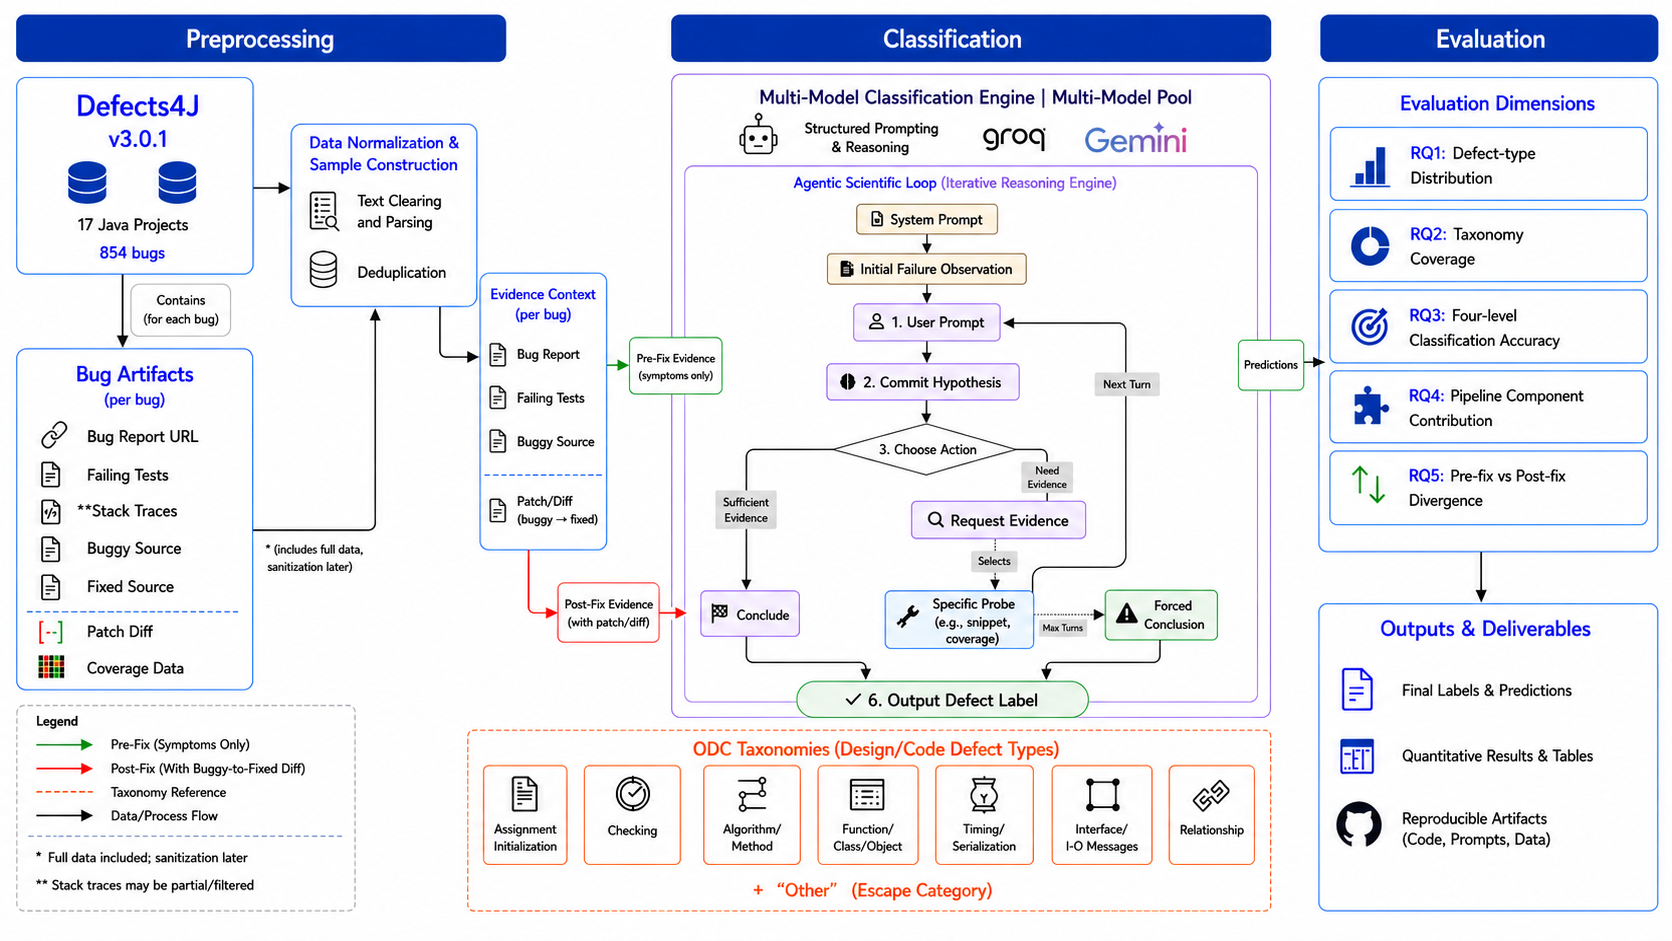
\includegraphics[width=\linewidth]{methodology_overview.png}
    \caption{Overview of the proposed methodology: preprocessing of Defects4J artifacts into per-bug evidence contexts, ODC classification through the agentic scientific loop, and evaluation across the five research questions}
    \label{fig:methodology}
\end{figure}

At the coarsest level the pipeline is the three-stage chain of Figure~\ref{fig:pipeline_stages}: Defects4J artifacts become a per-bug evidence file, that file becomes a classification, and the two classifications of the same bug become a comparison.

\begin{figure}[H]
\centering
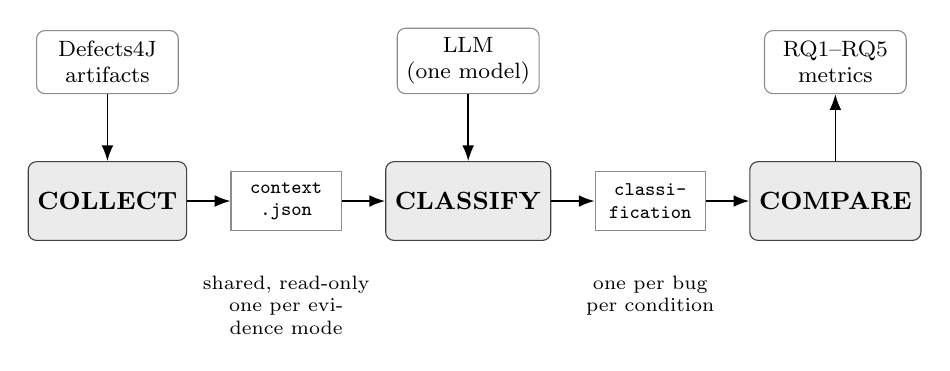
\begin{tikzpicture}[
  font=\small,
  stage/.style={rectangle, rounded corners=3pt, draw=black!75, fill=black!8,
                minimum width=2.0cm, minimum height=1.0cm, align=center},
  art/.style={rectangle, draw=black!45, fill=white, minimum width=1.4cm,
              minimum height=0.75cm, align=center, font=\scriptsize\ttfamily},
  src/.style={rectangle, rounded corners=3pt, draw=black!45, fill=white,
              minimum width=1.8cm, minimum height=0.8cm, align=center,
              font=\footnotesize},
  ar/.style={-{Latex[length=2mm]}, semithick}
]
\node[stage] (col) {\textbf{COLLECT}};
\node[art, right=0.55cm of col] (ctx) {context\\.json};
\node[stage, right=0.55cm of ctx] (cls) {\textbf{CLASSIFY}};
\node[art, right=0.55cm of cls] (cf) {classi-\\fication};
\node[stage, right=0.55cm of cf] (cmp) {\textbf{COMPARE}};

\draw[ar] (col) -- (ctx);
\draw[ar] (ctx) -- (cls);
\draw[ar] (cls) -- (cf);
\draw[ar] (cf) -- (cmp);

\node[src, above=0.85cm of col] (d4j) {Defects4J\\artifacts};
\draw[ar] (d4j) -- (col);

\node[src, above=0.85cm of cls, align=center] (llm) {LLM\\(one model)};
\draw[ar] (llm) -- (cls);

\node[src, above=0.85cm of cmp, align=center] (met) {RQ1--RQ5\\metrics};
\draw[ar] (cmp) -- (met);

\node[font=\scriptsize, below=0.45cm of ctx, align=center, text width=2.2cm]
  {shared, read-only\\one per evidence mode};
\node[font=\scriptsize, below=0.45cm of cf, align=center, text width=2.2cm]
  {one per bug\\per condition};
\end{tikzpicture}
\caption{The three pipeline stages and the artifacts that pass between them. The filesystem is the contract: each stage reads and writes JSON, so any stage can be rerun or audited independently.}
\label{fig:pipeline_stages}
\end{figure}

The three stages are:

\begin{enumerate}
    \item \textbf{Preprocessing.} We build the bug a case file: the report, the failing tests, the error messages, and the code around them. This is exactly what a developer would look at before reading the fix. The output is a structured \texttt{context.json} per bug.
    \item \textbf{Classification.} We hand that case file to a large language model and ask it to assign an ODC defect type, using one of three prompting strategies that range from a single quick guess to an enforced, evidence-driven reasoning loop. The output is a \texttt{classification.json} per bug per condition.
    \item \textbf{Evaluation.} Because Defects4J carries no official ODC answer key, we check the classification against itself under better information: we classify the same bug a second time after showing the model the real fix, and measure how closely the early, symptom-only classification matches the later, fix-informed one.
\end{enumerate}

Two architectural principles hold throughout. First, \textbf{multi-provider LLM support}: the pipeline abstracts over Gemini, OpenRouter, Groq, and OpenAI-compatible APIs, so the classification logic is independent of any one vendor. Second, \textbf{hidden oracle exclusion}: the list of classes the fix actually modified is stored separately and never enters the LLM-facing prompt, so the pre-fix arm cannot leak fix knowledge \cite{rafi2024revisiting}.

\section{ODC and Defects4J Artifact Mapping}

Before describing the collection process, it helps to see why Defects4J and ODC fit together as well as they do. ODC's two-phase opener/closer model maps onto the Defects4J artifact set almost directly.

Figure~\ref{fig:odc_mapping} shows the mapping, and the rest of this section explains each edge.

\begin{figure}[H]
\centering
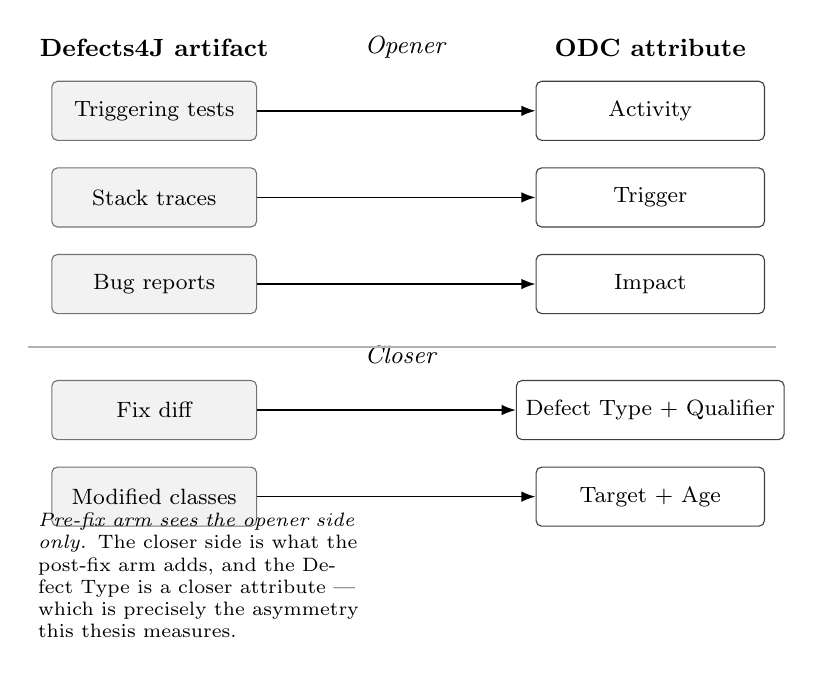
\begin{tikzpicture}[
  font=\footnotesize,
  art/.style={rectangle, rounded corners=2pt, draw=black!55, fill=black!5,
              minimum width=2.6cm, minimum height=0.75cm, align=center},
  odc/.style={rectangle, rounded corners=2pt, draw=black!75, fill=white,
              minimum width=2.9cm, minimum height=0.75cm, align=center},
  ar/.style={-{Latex[length=1.8mm]}, semithick},
  hdr/.style={font=\small\bfseries}
]
\node[hdr] at (0,1.35)   {Defects4J artifact};
\node[hdr] at (6.3,1.35) {ODC attribute};

% opener
\node[art] (t)  at (0, 0.55)  {Triggering tests};
\node[art] (st) at (0,-0.55)  {Stack traces};
\node[art] (br) at (0,-1.65)  {Bug reports};
\node[odc] (ac) at (6.3, 0.55) {Activity};
\node[odc] (tr) at (6.3,-0.55) {Trigger};
\node[odc] (im) at (6.3,-1.65) {Impact};
\draw[ar] (t)  -- (ac);
\draw[ar] (st) -- (tr);
\draw[ar] (br) -- (im);

% closer
\node[art] (df) at (0,-3.25)  {Fix diff};
\node[art] (mc) at (0,-4.35)  {Modified classes};
\node[odc] (dt) at (6.3,-3.25) {Defect Type $+$ Qualifier};
\node[odc] (tg) at (6.3,-4.35) {Target $+$ Age};
\draw[ar] (df) -- (dt);
\draw[ar] (mc) -- (tg);

% group labels
\node[font=\small\itshape, anchor=west] at (2.55, 1.35) {Opener};
\node[font=\small\itshape, anchor=west] at (2.55,-2.55) {Closer};
\draw[black!30] (-1.6,-2.45) -- (7.9,-2.45);

\node[font=\scriptsize, anchor=west, text width=4.2cm] at (-1.6,-5.35)
  {\textit{Pre-fix arm sees the opener side only.} The closer side is what the
   post-fix arm adds, and the Defect Type is a closer attribute --- which is
   precisely the asymmetry this thesis measures.};
\end{tikzpicture}
\caption{The natural mapping between Defects4J artifacts and ODC opener/closer attributes. Impact is shown for completeness; this study classifies Defect Type only (Section~\ref{sec:impact}).}
\label{fig:odc_mapping}
\end{figure}

On the \textbf{opener} side, which is the discovery story:

\begin{itemize}
    \item \textbf{Tests} map to \textbf{Activity}, because the test type tells us what was being performed when the defect was found. For Defects4J this is a unit test in every case.
    \item \textbf{Stack traces} map to \textbf{Trigger}, because the runtime context captured in the trace shows the specific condition that exposed the dormant defect.
    \item \textbf{Bug reports} map to \textbf{Impact}, because they describe the user-visible symptom and consequence, such as a crash or a wrong result.
\end{itemize}

On the \textbf{closer} side, which is the repair story:

\begin{itemize}
    \item \textbf{Code diffs} map to \textbf{Defect Type} and \textbf{Qualifier}, because the diff reveals the semantic nature of the mistake and how it manifested (Missing, Incorrect, or Extraneous).
    \item \textbf{Modified classes} map to \textbf{Target} and \textbf{Age}, because they show where the fix was applied and, with commit history, when the defect was likely injected.
\end{itemize}

Two of ODC's eight attributes are fixed by how the dataset is built rather than classified. \textbf{Target} is always Code, because Defects4J bugs are fixed in source and there is no separate design document. \textbf{Source} would be Developed In-House for nearly every project, since these are long-running community-maintained Java libraries.

This clean separation is not incidental. It enforces ODC's own design principle that subjective discovery data is never mixed with objective technical repair data \cite{chillarege1992odc}. It is also precisely what makes our evaluation possible: the pre-fix arm sees opener evidence, the post-fix arm additionally sees closer evidence, and the defect type is a closer attribute. That asymmetry is the thing we measure.

\section{Preprocessing and Evidence Collection}
\label{sec:collection}

In this study, we classify defects using pre-fix evidence, consisting of the information available before the defect is repaired, including the bug report, failing tests, stack traces, and relevant source-code context. To evaluate the resulting classifications in the absence of ground-truth ODC annotations in Defects4J, we additionally perform a post-fix evaluation, in which the model is provided with the corresponding fix information as an evaluation reference.

To classify a Defects4J bug into an ODC type using an LLM, we prepare two types of file: a \textbf{pre-fix context} and a \textbf{post-fix context}, for the buggy and the fixed version of the code respectively. The only difference between these two files is the \textbf{fix diff}, which represents the exact difference between a buggy version of the code and its fixed version. These two files are fed to an LLM to provide the context necessary to classify the bug automatically.

Bug classification should be performed solely using the pre-fix context, without access to any information from the corresponding fix. Since the Defects4J dataset does not include ground-truth ODC defect-type labels, we evaluate our approach by using the post-fix context, where the actual code changes provide sufficient evidence for defect-type classification.

The preprocessing stage gathers this multi-modal bug information from Defects4J and normalizes it into one file per bug per evidence mode. For each bug we extract and store the following artifacts as the context the LLM uses to classify the bug.

\paragraph{Bug identity and Defects4J metadata.} We record the project and bug IDs, the buggy and fixed revision hashes, the issue-tracker report ID and URL, the modified classes, and the triggering and relevant tests.

\paragraph{Bug report content.} We fetch the original bug report from the issue tracker (JIRA, GitHub, or a generic web page) and store it in full, including its title, labels, and comment thread.

\paragraph{Failing tests, exception, and stack trace.} We check out the buggy revision, compile it, and run the test suite to confirm the bug still reproduces. For each triggering test we capture its name, the raised exception, the raw stack trace, and a parsed list of every frame with its class, method, file, and line.

\paragraph{Suspicious frames.} A raw Java stack trace is mostly noise. A single failing JUnit test typically produces thirty to sixty frames, of which the large majority belong to the test harness (JUnit, TestNG, Hamcrest), the JDK (\texttt{java.lang}, \texttt{java.util}, reflection internals), or the build tool (Ant, Maven). None of those frames says anything about the defect.

A \textbf{suspicious frame} is a stack frame that points into the project's own source tree. We identify them by filtering the parsed frame list against the project's source roots and discarding everything outside them, preserving the original stack order so the innermost project frame comes first. Suspicious frames matter for two reasons. They are the anchor points for snippet extraction described below, so they decide which code the model actually gets to read; and their ordering encodes the call path that led to the failure, which is diagnostic information in its own right. Getting this filter right is what separates a case file the model can reason over from a wall of framework internals.

\paragraph{Code snippets.} Around each suspicious frame and each failing test we cut a short source window with the offending line marked. Production snippets take $\pm$12 lines around the frame; test snippets take $\pm$18 lines, because a test's assertion is usually further from its setup. This gives localized context showing expected versus actual behaviour.

\paragraph{Coverage (optional).} We can run Cobertura-style coverage analysis on the suspicious classes and parse the resulting XML for line and branch execution rates. This is available to the model as a probe target rather than included by default.

\paragraph{Normalization and deduplication.} Raw artifacts are not directly usable. Bug report HTML is stripped to text, tracker boilerplate and signature blocks are removed, and whitespace is collapsed, so that the same report does not consume different amounts of prompt budget depending on its source tracker. Stack traces are deduplicated in two ways: repeated frames from recursive calls are collapsed, and when several triggering tests produce the same trace prefix, the shared prefix is stored once rather than repeated per test. Code snippets are deduplicated by source range, so two suspicious frames landing in the same method do not yield two overlapping copies of it. The effect is that the case file contains each distinct piece of evidence exactly once, which both reduces prompt size and prevents the model from reading a repeated frame as additional evidence.

\paragraph{Hidden oracles.} We separately store the modified classes as a hidden oracle. This field is excluded from the LLM-facing prompt in both arms and used only during evaluation, for example to check whether a probe actually reached the buggy class.

\paragraph{Fix diff (post-fix oracle).} For post-fix evaluation we also record the buggy-to-fixed source diff. This field is empty in the pre-fix record and withheld from the model otherwise.

\paragraph{Keeping the fix out of the pre-fix evidence.} A pre-fix classification is only meaningful if it genuinely cannot see the fix, and two channels can leak fix knowledge by accident. First, the raw Defects4J metadata names the classes the fix touched. Second, bug-report text for already-resolved issues often discusses the resolution, with status transitions and ``fixed in'' comments. We strip both from the pre-fix evidence immediately before it is shown to the model, while leaving the post-fix evidence untouched, since that arm is allowed to know the fix. The result is two versions of the same case file that differ in exactly one respect, which is precisely what the pre-fix/post-fix comparison is designed to isolate.

\section{Evidence Modes: Pre-fix versus Post-fix}

The pipeline operates in two evidence modes.

\textbf{Pre-fix mode} is the default and gives the model only symptoms: stack traces, test failures, error messages, code snippets, and bug report content. The model sees what went wrong and must reason about the root cause without knowing the fix. This mirrors opener-side ODC evidence. Conceptually, it is like a doctor diagnosing a patient from symptoms alone.

\textbf{Post-fix mode} additionally supplies the actual buggy-to-fixed code diff. The model can now see exactly what was changed, which is closer-side ODC evidence. This is like a pathologist with the biopsy results.

ODC's opener/closer model naturally requires evidence from both perspectives \cite{chillarege1992odc}. The dual-mode design is what enables evaluation without ground truth: if the pipeline classifies well from symptoms alone, the pre-fix result should broadly reproduce the post-fix result.

\section{The Condition Space: Taxonomy and Strategy}
\label{sec:conditions}

A single prompt bundles together two decisions that ought to be separated: \emph{what label space} the model may answer in, and \emph{how} it is asked to reason toward an answer. We separate them into two independent axes, which is what makes the RQ4 ablation possible.

\subsection{The Taxonomy Axis: How Strict the Vocabulary Is}

\begin{itemize}
    \item \textbf{free} --- the model answers in its own words with no fixed list at all. This lets us later measure how much a taxonomy narrows down an otherwise sprawling vocabulary.
    \item \textbf{closed} --- the model must pick exactly one of the seven canonical ODC Design/Code types.
    \item \textbf{open} --- the model may pick one of the seven, or say ``Other'', but an escape is only accepted together with a written justification, its best guess at the nearest of the seven types, and a confidence score. Every escape is therefore auditable rather than a shrug.
\end{itemize}

\textbf{Open is our default.} The reason is a methodological commitment: we never force-fit a bug into a fixed schema. If a defect genuinely does not belong to any ODC type, that is data we want to record, not an error to hide. Section~\ref{sec:rq2} reports what happened when we offered that escape.

\subsection{The Strategy Axis: How the Model Reasons}

\paragraph{Zero: a single quick guess.} One plain prompt, no taxonomy, no examples. This is the unstructured baseline every other strategy is measured against. By definition it is taxonomy-free, because a model given no list cannot be constrained to one.

\paragraph{Few: one strong, well-prepared prompt.} The second strategy still asks for a single answer, but the prompt is built carefully. It defines every ODC type with example patterns, warns the model away from defaulting to the vague catch-all Function/\allowbreak Class/\allowbreak Object type, walks through a short decision checklist before that catch-all is even allowed to be considered, and includes worked examples chosen specifically for pairs of types that are easy to confuse. This is the strongest single-shot prompt we could build, and it is deliberately the fair baseline the third strategy has to beat.

\paragraph{Scientific: an enforced reasoning loop.} The third strategy does not let the model narrate a chain of thought and call it done. Section~\ref{sec:loop} describes it in full.

\subsection{Five Valid Conditions of Nine}

Not every cell of the $3 \times 3$ grid is meaningful. A zero-shot prompt carries no vocabulary constraint, and the free setting defines none, so only five combinations are valid. Figure~\ref{fig:conditions} shows the space.

\begin{figure}[H]
\centering
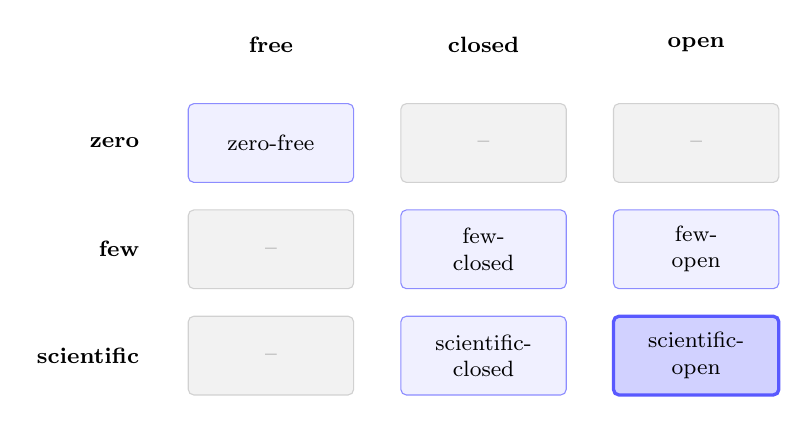
\begin{tikzpicture}[
  font=\footnotesize,
  cell/.style={rectangle, rounded corners=2pt, minimum width=2.1cm,
               minimum height=1.0cm, align=center, draw},
  valid/.style={cell, fill=blue!6,  draw=blue!45},
  def/.style={cell,   fill=blue!18, draw=blue!65, very thick},
  invalid/.style={cell, fill=black!5, draw=black!18, text=black!45},
  hdr/.style={align=center, font=\footnotesize\bfseries}
]
% column headers (taxonomy)
\node[hdr] at (0,1.25)   {free};
\node[hdr] at (2.7,1.25) {closed};
\node[hdr] at (5.4,1.25) {open};
% row headers (strategy)
\node[hdr, anchor=east] at (-1.55, 0)    {zero};
\node[hdr, anchor=east] at (-1.55,-1.35) {few};
\node[hdr, anchor=east] at (-1.55,-2.70) {scientific};
% grid
\node[valid]   at (0,0)      {zero-free};
\node[invalid] at (2.7,0)    {--};
\node[invalid] at (5.4,0)    {--};
\node[invalid] at (0,-1.35)  {--};
\node[valid]   at (2.7,-1.35){few-\\closed};
\node[valid]   at (5.4,-1.35){few-\\open};
\node[invalid] at (0,-2.70)  {--};
\node[valid]   at (2.7,-2.70){scientific-\\closed};
\node[def]     at (5.4,-2.70){scientific-\\open};
\end{tikzpicture}
\caption{The three classification strategies (rows) crossed with the three vocabulary settings (columns). Five of the nine cells are valid; the four grey cells are invalid combinations, since \textit{zero} carries no vocabulary constraint and \textit{free} defines none. \textit{scientific-open} (bold) is the default for both pre-fix and post-fix evidence.}
\label{fig:conditions}
\end{figure}

We settled on \textbf{scientific-open} as the default for two reasons. First, forcing every bug into a fixed seven-type list manufactures false certainty for bugs that genuinely do not fit, so the open vocabulary turns taxonomy coverage into something we measure rather than assume. Second, in early testing, simply \emph{narrating} a step-by-step reasoning style left the model's answers unchanged; only when that reasoning was \emph{enforced}, forcing a committed prediction before new evidence was revealed, did a meaningful share of labels actually change, and they moved toward the fix-informed reference.

\section{Prompt Design}

Every classification uses two prompts with distinct jobs.

\textbf{The system prompt carries everything that is constant across bugs.} It defines the task, the ODC taxonomy with per-type definitions and contrastive ``distinguish from'' guidance, the anti-bias rules, the diagnostic decision tree, the required output schema, and the worked examples. It is the model's rulebook, and it is byte-identical for every bug within a condition. That constancy is what makes conditions comparable: any difference in output between two bugs comes from the evidence, not from the instructions.

\textbf{The user prompt carries everything specific to one bug.} It is the evidence payload: the bug report text, the failing tests, the exception and stack trace, the suspicious frames, and the code snippets, with hidden oracles filtered out and, in post-fix mode, the fix diff appended. It contains no instructions at all.

The system prompt is assembled from six components:

\begin{enumerate}
    \item \textbf{ODC taxonomy.} The seven defect types with definitions, diagnostic indicators, and contrastive guidance that helps the model differentiate similar types.
    \item \textbf{Anti-bias rules.} Explicit instructions not to default to Function/\allowbreak Class/\allowbreak Object, the most general structural type, and to consider simpler explanations first. The rule names no expected distribution, so it cannot bias the very distribution RQ1 measures.
    \item \textbf{Reasoning protocol.} Either the enforced loop of Section~\ref{sec:loop} or, in the \emph{few} condition, the static decision checklist.
    \item \textbf{Diagnostic decision tree.} Seven questions, each mapping to one ODC type. Function/\allowbreak Class/\allowbreak Object is deliberately placed last, to force consideration of simpler types first.
    \item \textbf{JSON schema.} A structured output format requiring the chosen type, close alternatives, the ODC family, a confidence score, a reasoning trace, and, where applicable, the escape justification.
    \item \textbf{Few-shot examples.} Contrastive examples following the pattern symptom, code, classification, and why it is \emph{not} the neighbouring type \cite{koyuncu2025exploring}.
\end{enumerate}

\section{The Enforced Scientific Reasoning Loop}
\label{sec:loop}

The loop is the core of our contribution, and it is worth being precise about what it does and where it comes from.

Zeller's scientific debugging \cite{zeller2009why} is a \emph{process}: observe the failure, form a hypothesis consistent with what you observed, predict what else must be true if the hypothesis holds, run an experiment or examine the code to test that prediction, and conclude. \textcite{kang2023autosd} adapted this to LLM prompting for fault localization, where the initial failure observation, meaning the failing test, error message, and code, is the \emph{prompt input}, and each subsequent iteration runs a tight cycle.

We adopt the AutoSD loop-iteration structure and adapt it from localizing a fault to naming its type. In our pipeline the initial failure observation is the evidence context, and on every turn the model must:

\begin{enumerate}
    \item \textbf{Hypothesis.} Commit to a specific claim about the defect type, in writing, before seeing anything new.
    \item \textbf{Prediction.} State what specific evidence would have to be true if that hypothesis were correct.
    \item \textbf{Experiment.} Request exactly that piece of evidence from the case file, by issuing a probe for a code snippet, a coverage figure, a test source, or a stack frame it has not yet been shown.
    \item \textbf{Observation.} Read what actually came back. The probe's real return payload is recorded verbatim in the transcript, truncated to 2{,}000 characters.
    \item \textbf{Conclusion.} Judge whether the observation supports or contradicts the hypothesis, and either conclude or begin another turn, to a maximum of six.
\end{enumerate}

Figure~\ref{fig:loop} shows the cycle. The initial failure observation enters once, as the prompt input; the dashed edge is the path taken when the evidence gathered so far is not yet sufficient to conclude.

\begin{figure}[H]
\centering
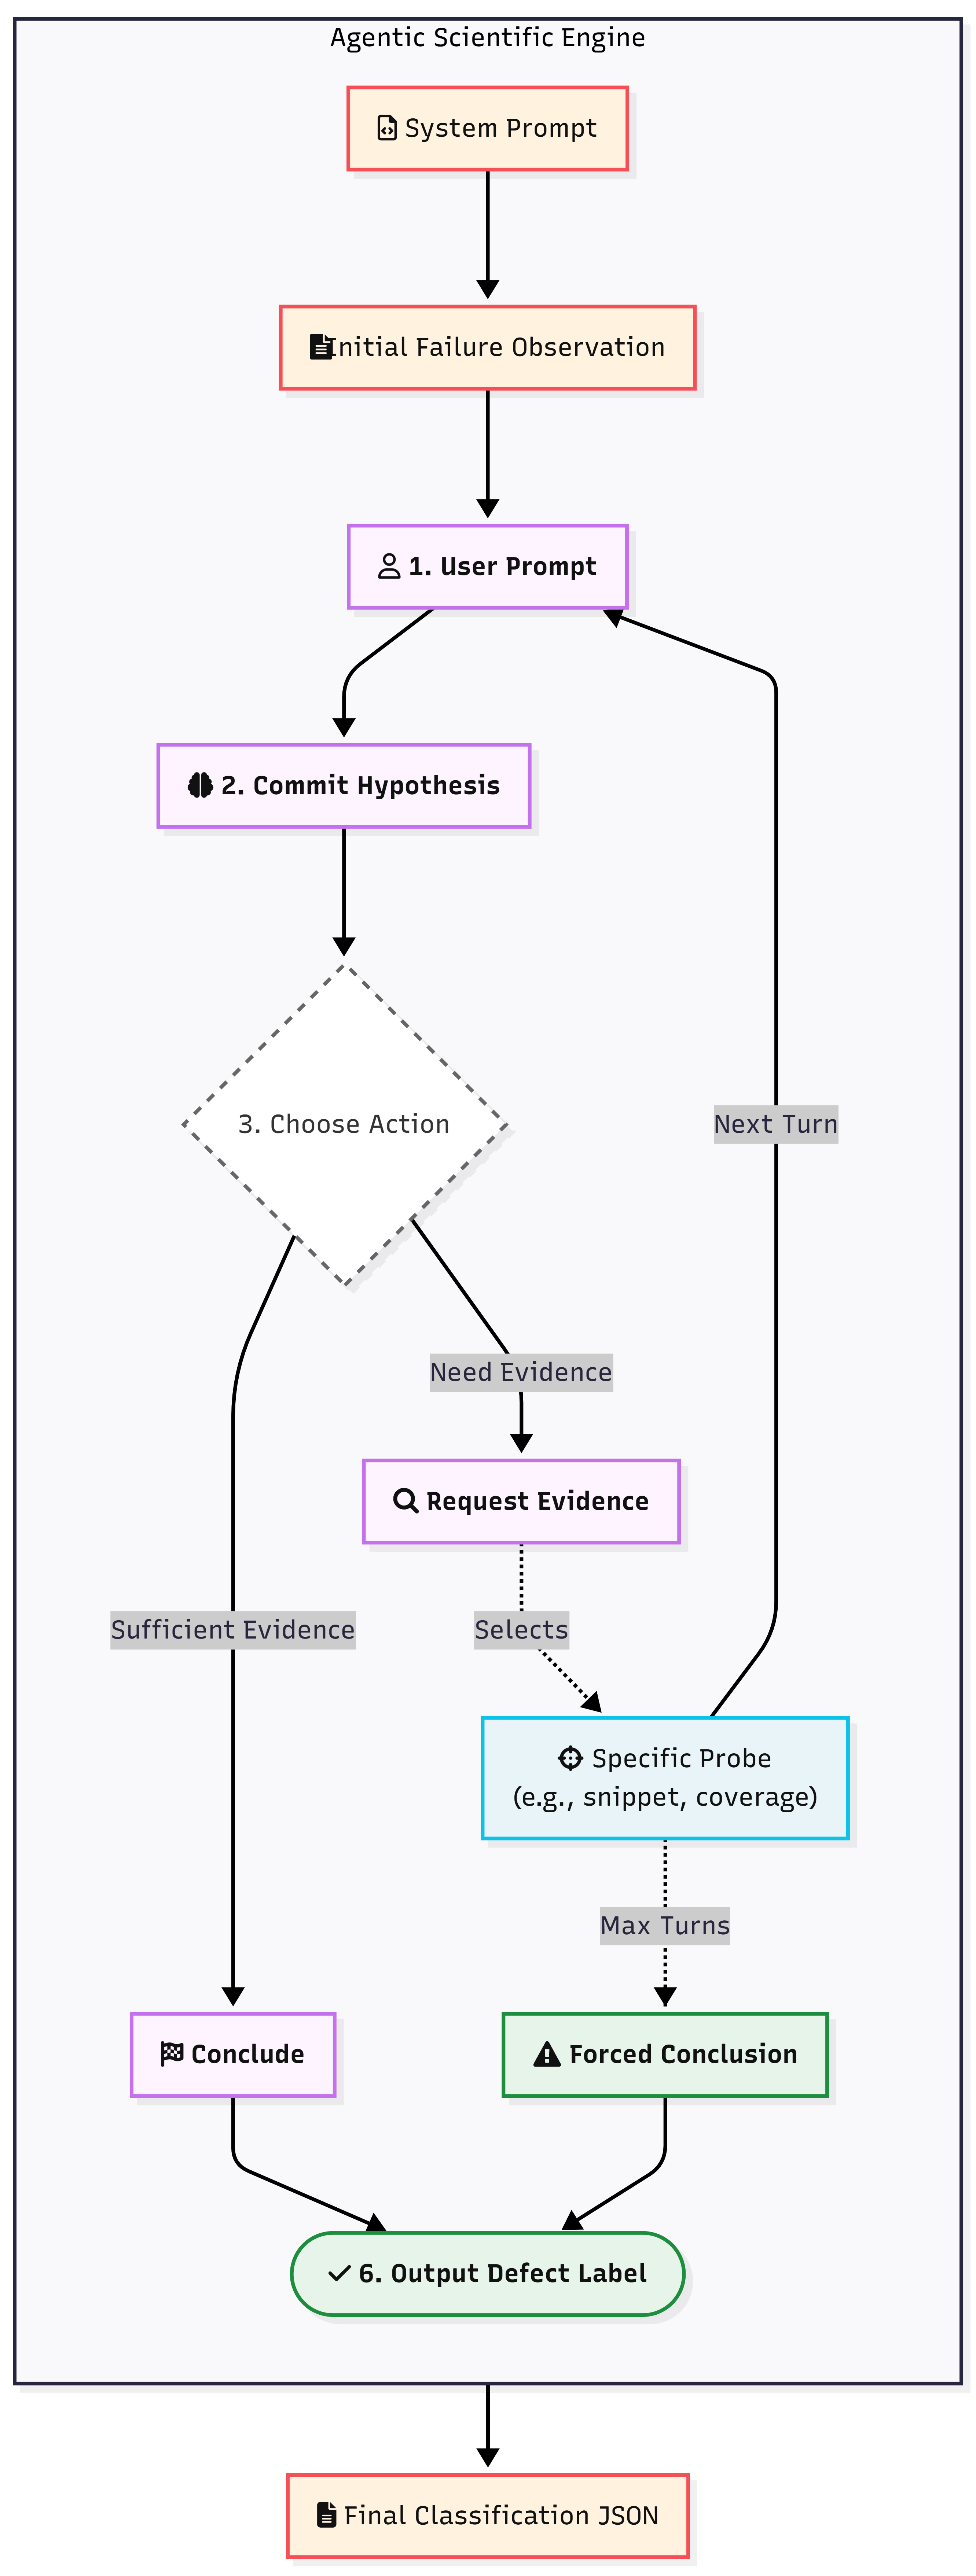
\includegraphics[width=0.6\linewidth]{scientificloop.png}
\caption{The enforced reasoning loop, adapted from the AutoSD loop-iteration structure \cite{kang2023autosd}. The failure observation is the prompt input; each turn then runs hypothesis, prediction, experiment, observation, conclusion.}
\label{fig:loop}
\end{figure}

The ordering matters and is not interchangeable. Because the model must commit to a prediction \emph{before} it is allowed to see the evidence that would confirm or deny it, the strategy cannot simply rationalise a first guess after the fact. That is exactly what distinguishes it from a narrated chain of thought, where the model produces reasoning and conclusion together and the reasoning can be written to fit the conclusion.

If the loop reaches its turn limit without concluding, the model is forced to conclude from what it has, and this is recorded as a forced conclusion rather than presented as a normal one. Every turn, every probe, every returned payload, and every hypothesis revision is written into the classification artifact, so the entire reasoning chain is auditable after the fact. Section~\ref{sec:rq4b} uses those transcripts to measure how often the loop actually reached the buggy code.

\subsection{A Worked Turn}

An abstracted example makes the mechanism concrete. Consider a bug whose only visible symptom is an assertion failure comparing two numeric values, with a stack trace pointing into a utility method.

\begin{description}
    \item[Hypothesis.] ``The defect is \emph{Checking}: the method does not guard against an empty input range, so it proceeds into a computation that is undefined for that input.''
    \item[Prediction.] ``If that is right, the method body will contain an arithmetic expression over the range with no preceding emptiness or bounds test.''
    \item[Experiment.] The model issues a probe for the source of the named method. It has not been shown that source yet.
    \item[Observation.] The returned snippet contains a bounds test, but the arithmetic that follows uses the wrong comparison operator.
    \item[Conclusion.] The prediction is refuted. The guard exists. The model revises to \emph{Algorithm/Method} and, on the next turn, probes the failing test to confirm the expected value is consistent with a corrected operator.
\end{description}

The important property is not that the model reached the right answer. It is that the hypothesis was written down, in a specific and falsifiable form, \emph{before} the evidence that refuted it was requested. A narrated chain of thought produces its reasoning and its conclusion in the same generation step, which means the reasoning can be written to justify whatever conclusion the model was already going to reach. Here it cannot, because the observation arrives from the evidence store after the prediction is fixed. This distinction is what the ablation in Section~\ref{sec:rq4b} measures.

\section{Output Validation}

Whatever the model returns is checked before it is trusted. We confirm the type is one of the seven canonical names or a properly justified ``Other''; clamp the confidence score into range; \textbf{recompute the ODC family from the chosen type ourselves} rather than trusting the model's own labelling; and normalize the alternative-type and reasoning fields so every downstream artifact has the same shape. Transient HTTP errors (429, 500, 502, 503) are retried with exponential backoff. This validation layer keeps a malformed or internally inconsistent answer from quietly corrupting the aggregate results.

Filenames are condition-tagged (\texttt{classification.<strategy>-<taxonomy>.json}) and written beside the shared, read-only \texttt{context.json}, so every condition reuses one evidence store and no condition can overwrite another.

\section{The Evaluation Framework}
\label{sec:eval}

Since Defects4J does not provide ground-truth ODC defect-type annotations, we use the post-fix classification as a \emph{fix-informed reference} for evaluating the pre-fix prediction. The fix provides additional evidence about the nature of the defect, allowing us to examine whether the classification inferred from symptoms and code context remains consistent when the actual repair is revealed.

The last step therefore asks a simple question: how much do we trust the classification? Defects4J gives us no official ODC answer key, so instead of measuring against ground truth, we measure a classification against itself under better information. We take the pre-fix classification, which saw symptoms only, and compare it with the post-fix classification of the same bug, which additionally saw the real fix.

\subsection{What ``Accuracy'' Can and Cannot Mean Here}

We have to be honest about this from the start, because the rest of the evaluation depends on it. \textbf{Defects4J has no ODC labels.} Nobody has ever labelled these bugs with ODC defect types, so there is no answer key, and ``accuracy against ground truth'' is not a quantity that exists for this dataset.

What we do instead is construct the best available \textbf{reference standard} and measure against it. Our reference is the post-fix run: the same model, the same taxonomy, the same prompt, on the same bug, but with the developer's actual fix diff included in the evidence. The question then becomes precise and answerable: \emph{how often does the pre-fix run produce the same label as the fix-aware run?}

Three things justify treating the post-fix arm as the reference:

\begin{enumerate}
    \item \textbf{It sees the evidence that defines the answer.} An ODC defect type describes the nature of the corrective change. The post-fix run sees that change; the pre-fix run has to infer it. When the defining evidence is present, the label is better grounded.
    \item \textbf{It is the standard move when no ground truth exists.} This is a two-rater design in which the second rater is deliberately given more information. Reporting agreement with a better-informed rater is what inter-rater reliability studies do, and Section~\ref{sec:human_agreement} shows that ODC agreement is exactly this evidence-dependent.
    \item \textbf{Our data confirms the post-fix arm is the more stable one.} The human-review flag fires 11 times in the pre-fix arms and zero times in either post-fix arm. The two strategies also agree with each other substantially more in post-fix than in pre-fix. Give both strategies the fix and they converge; take it away and they diverge, which is what you expect if the fix resolves ambiguity.
\end{enumerate}

\subsection{The Four Levels}

We grade agreement at four levels of strictness, from strictest to most forgiving.

\begin{enumerate}
    \item \textbf{Level 1 --- Strict match.} Do the pre-fix and post-fix classifications assign the exact same ODC type? This is the headline metric.
    \item \textbf{Level 2 --- Cohen's $\kappa$.} The same question, corrected for the agreement you would get by chance. This matters because a classifier that puts most bugs in one category gets a high raw agreement for free; $\kappa$ prices that in.
    \item \textbf{Level 3 --- Top-2 match.} Does the other run's primary type appear in this run's list of close alternatives? This captures cases where the model recognized the right type but ranked it second.
    \item \textbf{Level 4 --- Family match.} Do both labels fall in the same ODC family, Control and Data Flow or Structural? This captures broad semantic agreement when the specific type differs.
\end{enumerate}

Figure~\ref{fig:eval_levels} arranges them as a ladder from strictest to most forgiving.

\begin{figure}[H]
\centering
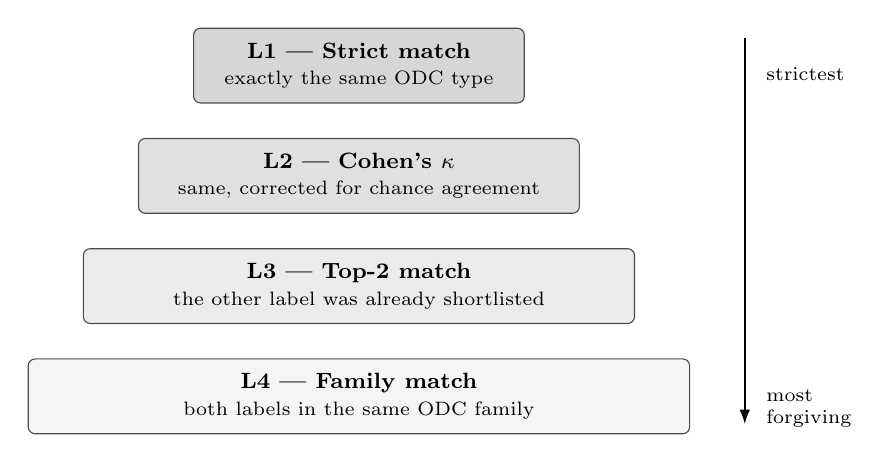
\begin{tikzpicture}[
  font=\footnotesize,
  lvl/.style={rectangle, rounded corners=2.5pt, draw=black!70,
              minimum height=0.95cm, align=center},
  ar/.style={-{Latex[length=1.8mm]}, semithick}
]
\node[lvl, fill=black!16, minimum width=4.2cm]  (l1) at (0, 0)     {\textbf{L1 --- Strict match}\\\scriptsize exactly the same ODC type};
\node[lvl, fill=black!12, minimum width=5.6cm]  (l2) at (0,-1.40)  {\textbf{L2 --- Cohen's $\kappa$}\\\scriptsize same, corrected for chance agreement};
\node[lvl, fill=black!8,  minimum width=7.0cm]  (l3) at (0,-2.80)  {\textbf{L3 --- Top-2 match}\\\scriptsize the other label was already shortlisted};
\node[lvl, fill=black!4,  minimum width=8.4cm]  (l4) at (0,-4.20)  {\textbf{L4 --- Family match}\\\scriptsize both labels in the same ODC family};

\draw[ar] (4.9, 0.35) -- (4.9,-4.55);
\node[font=\scriptsize, anchor=west, align=left] at (5.05,-0.1)  {strictest};
\node[font=\scriptsize, anchor=west, align=left] at (5.05,-4.35) {most\\forgiving};
\end{tikzpicture}
\caption{The four-level evaluation framework. Each level relaxes the agreement criterion, and the widening bars indicate that each level admits everything the level above it admits. Levels 3 and 4 sit near their own ceiling and must be read conditional on Level 1 having failed --- see Section~\ref{sec:l3l4}.}
\label{fig:eval_levels}
\end{figure}

Cohen's $\kappa$ is computed as
\begin{equation}
    \kappa = \frac{p_o - p_e}{1 - p_e},
    \label{eq:kappa}
\end{equation}
where $p_o$ is the observed agreement and $p_e$ the agreement expected by chance alone, and is read on the standard Landis--Koch scale, where $0.41$--$0.60$ counts as moderate and $\kappa \geq 0.61$ as substantial \cite{landis1977measurement}.

\subsection{How Levels 3 and 4 Must Be Read}
\label{sec:l3l4}

There is a trap in this framework that we want to disarm before presenting results, because a reviewer will otherwise spot it.

Levels 3 and 4 produce high numbers, but they sit close to their own ceiling. If you shuffle our labels at random, the top-2 and family match rates are still around 90\%, simply because three types dominate the benchmark and all three belong to the same family. Quoted on their own, those two numbers carry almost no information.

\textbf{The fix is to read them as severity, not as accuracy.} They are not four independent accuracy tests. Levels 3 and 4 describe \emph{how bad the disagreement is on the bugs where Level 1 already failed}. We therefore report them conditional on disagreement throughout Chapter~\ref{chapter:results}, which turns two near-ceiling numbers into a meaningful measure of how far apart the two labels actually are.

\section{Summary}

The methodology combines three ideas: multi-modal evidence collected from Defects4J into a normalized case file, ODC's principled taxonomy with an explicit escape category, and an enforced hypothesis-and-probe loop adapted from scientific debugging. Separating the taxonomy axis from the strategy axis gives a controlled condition space, and the dual-mode pre-fix/post-fix design provides an evaluation reference in a benchmark that has no labels. The next chapter describes the experimental setup, and Chapter~\ref{chapter:results} reports what all of this produced.


% ================================================================
% CHAPTER 5: EXPERIMENTAL DESIGN / DATA COLLECTION
% ================================================================
\chapter{Experimental Design and Data Collection} \label{chapter:experiment}

This chapter describes how we set up the experiments, what data we collected, how the pipeline was configured, and which statistical methods we used to analyse the results.

\section{Dataset: Defects4J}

The experiments use Defects4J v2.0, which contains over 830 active bugs across 17 open-source Java projects \cite{just2014defects4j}. Table~\ref{tab:d4j_projects} lists them.

\begin{table}[H]
    \centering
    \begin{tabular}{l l r}
        \toprule
        \textbf{Project} & \textbf{Description} & \textbf{Active Bugs} \\
        \midrule
        Chart & JFreeChart plotting library & 26 \\
        Cli & Apache Commons CLI & 40 \\
        Closure & Google Closure Compiler & 174 \\
        Codec & Apache Commons Codec & 18 \\
        Collections & Apache Commons Collections & 4 \\
        Compress & Apache Commons Compress & 47 \\
        Csv & Apache Commons CSV & 16 \\
        Gson & Google Gson & 18 \\
        JacksonCore & Jackson JSON core & 26 \\
        JacksonDatabind & Jackson databinding & 112 \\
        JacksonXml & Jackson XML & 6 \\
        Jsoup & HTML parser & 93 \\
        JxPath & Apache JXPath & 22 \\
        Lang & Apache Commons Lang & 64 \\
        Math & Apache Commons Math & 106 \\
        Mockito & Mocking framework & 38 \\
        Time & Joda-Time & 26 \\
        \midrule
        \textbf{Total} & & \textbf{836} \\
        \bottomrule
    \end{tabular}
    \caption{Defects4J v2.0 projects and their approximate active bug counts. Per-project counts are version-dependent.}
    \label{tab:d4j_projects}
\end{table}

From this benchmark we pre-collected a shared evidence corpus of 854 pre-fix and 854 post-fix \texttt{context.json} payloads. Collecting this corpus took approximately one week of wall-clock time, because each bug requires a checkout, a compile, and a full test run. Every study run reuses this corpus, so no classification run triggers a fresh Defects4J checkout or test execution. This matters for reproducibility: the evidence is fixed, and only the classification varies.

\section{The Study Corpus}

The results reported in Chapter~\ref{chapter:results} come from \textbf{257 bugs across five projects}, shown in Table~\ref{tab:study_corpus}. These five were selected because they span the range of project characteristics in the benchmark: a plotting library, two general-purpose utility libraries, a numerical library, and a mocking framework, the last of which is far more interface-heavy than the rest.

\begin{table}[H]
    \centering
    \begin{tabular}{l r p{7.4cm}}
        \toprule
        \textbf{Project} & \textbf{Bugs} & \textbf{Character} \\
        \midrule
        Chart & 26 & Graphics and plotting; heavy object state \\
        Lang & 61 & String and utility functions; small, self-contained methods \\
        Math & 106 & Numerical algorithms; the largest and most computation-heavy \\
        Mockito & 38 & Mocking framework; interface- and proxy-heavy \\
        Time & 26 & Date and time arithmetic; boundary-condition heavy \\
        \midrule
        \textbf{Total} & \textbf{257} & \\
        \bottomrule
    \end{tabular}
    \caption{The five projects in the study corpus and why each was included}
    \label{tab:study_corpus}
\end{table}

Each of the 257 bugs was classified under two conditions in two evidence modes, giving $257 \times 2 \times 2 = 1{,}028$ classifications in the main dataset, plus a matching unstructured baseline over the same 257 bugs in both modes for RQ4a. Collection for the Closure project is ongoing and is not included in these results; this is stated explicitly as a threat to external validity in Chapter~\ref{chapter:threats}.

\section{Context File Structure}

Section~\ref{sec:collection} describes how each bug's case file is built; here we list exactly what it contains. Every \texttt{context.json} holds: the bug ID, project name, and report URL; failing-test summaries, exception messages, and stack-trace frames; production-code and failing-test snippets; optional Cobertura coverage summaries; hidden-oracle fields (the modified classes and the optional fix diff); and the buggy/fixed revision-pair metadata.

The file is deliberately a single self-describing artifact rather than a set of loose inputs. Three properties follow from that choice and matter for the study. First, \textbf{one context serves every condition}: the same \texttt{context.json} is read by the zero-shot baseline, the few-shot prompt, and the enforced loop, so no condition can be advantaged by having seen different evidence. Second, \textbf{the context is read-only during classification}, so a run cannot mutate the evidence another run will later use. Third, \textbf{the hidden-oracle fields travel with the file but never enter the prompt}, which means the evaluation layer can check what a probe reached without the classification layer ever being able to see it.

\section{Execution Environment}

Classifications ran against the Google Gemini API using the model \modelname, with schema-enforced structured output. \textbf{The same single model is used for every classification reported in this thesis}, so no result is confounded by a model change.

Defects4J tooling is invoked through WSL for the collection stage, but because all classification runs reuse the pre-collected corpus, the reported runs involve only LLM calls. Commands are scripted, dependency versions are pinned, and each run records context-reuse counts and per-classification turn and call counts.

\section{Evidence Collection Configuration}

Stack-frame filtering retains only project source frames, discarding JUnit, TestNG, Hamcrest, JDK-internal, and build-tool frames. Production snippets capture $\pm$12 lines around each suspicious frame. Test snippets capture $\pm$18 lines and are limited to the first three failing tests per bug. Coverage analysis is optional and focuses on the suspicious classes parsed from Cobertura XML. The enforced loop is capped at six turns, and each probe's return payload is truncated to 2{,}000 characters in the transcript.

\section{Condition Configuration}

Each research question fixes the conditions it needs. Table~\ref{tab:rqmap} maps every research question to the conditions it draws on and the metrics that answer it.

\begin{table}[H]
    \centering
    \begin{tabular}{l p{4.2cm} p{6.0cm}}
        \toprule
        \textbf{RQ} & \textbf{Conditions used} & \textbf{Metrics} \\
        \midrule
        RQ1 & scientific-open (all four reported) & Type distribution; per-project variation \\
        RQ2 & All open-taxonomy runs & Escape rate; coverage rate; escape upper bound \\
        RQ3 & scientific-open, few-open & Four levels: strict, $\kappa$, top-2, family \\
        RQ4a & zero-free vs few-open vs scientific-open & Unique labels; entropy; vocabulary reduction; label reproducibility \\
        RQ4b & few-open vs scientific-open & $\kappa$ difference; per-project $\kappa$; probe transcripts \\
        RQ5 & scientific-open, few-open & Drift transitions; per-project $\kappa$ with intervals \\
        \bottomrule
    \end{tabular}
    \caption{Research questions, the conditions each draws on, and the metrics that answer it}
    \label{tab:rqmap}
\end{table}

\section{Statistical Methods}
\label{sec:stats}

Several of our results rest on statistical tests, and a few standard tests would have been the wrong instrument here. This section states what we used and why, so that Chapter~\ref{chapter:results} can report results without interrupting itself to justify each test.

\paragraph{Monte Carlo permutation $\chi^2$ (RQ1).} The standard $\chi^2$ test of association assumes every cell has an expected count of at least five. Our project-by-type table violates that, because several ODC types are rare. We therefore shuffle the labels randomly across bugs 10{,}000 times and count how often a shuffled table is as uneven as ours. This needs no assumption about cell counts. We report Cram\'er's $V$ alongside it as an effect size.

\paragraph{Rule of three (RQ2).} A count of zero events does not admit a p-value, but it admits a bound. If zero events are observed in $n$ trials, the 95\% upper bound on the true rate is approximately $3/n$. This is how we convert ``no escapes were observed'' into a quantitative claim.

\paragraph{Bootstrap confidence intervals (RQ3, RQ5).} Per-project samples are small, with $n = 26$ for both Chart and Time, so a bare $\kappa$ point estimate is misleading. We resample bugs with replacement 2{,}000 times and report the resulting 95\% interval. Where an interval includes zero, we say so rather than quoting the point estimate alone.

\paragraph{Paired bootstrap on the $\kappa$ difference (RQ4b).} To compare two conditions evaluated on the \emph{same} bugs, we resample bugs, recompute both conditions' $\kappa$ on each resample, and take the difference. This preserves the pairing and gives a confidence interval on the difference itself, which is the quantity of interest. We use 5{,}000 resamples.

\paragraph{McNemar's exact test (RQ4a, RQ4b).} For paired binary outcomes, agreeing or not agreeing with the reference, McNemar's test compares the two discordant cells. We report it, but note where it and $\kappa$ disagree, and explain the mechanism, because McNemar counts raw agreement flips and ignores chance correction.

\paragraph{Sign test (RQ4b).} A non-parametric check on whether one condition beats another consistently across projects, independent of the size of each gain.

\paragraph{Total variation distance and entropy (RQ1, RQ4a, RQ5).} Total variation distance measures how far two label distributions are apart, on a scale from 0 to 1. Shannon entropy measures how spread out a single distribution is, in bits. We use TVD to compare distributions across conditions and modes, and entropy to quantify vocabulary collapse in the ablation.

\section{Data Provenance and Verification}

All figures reported in Chapter~\ref{chapter:results} were recomputed directly from the per-bug classification artifacts on disk, using the pipeline's own comparison functions, rather than from any intermediate summary. As an independent check, the five per-project analysis workbooks maintained alongside the study were cross-validated against the raw artifacts across all 257 bugs and all four conditions, with zero mismatches. Every classification artifact retains its full reasoning transcript, so any number in the next chapter can be traced back to the individual model outputs that produced it.


% ================================================================
% CHAPTER 6: RESULTS AND ANALYSIS
% ================================================================
\chapter{Results and Analysis} \label{chapter:results}

This chapter reports the results for all five research questions. For each, we state what the question asks, what we found, what the statistics say, and, importantly, what the result can and cannot be claimed to show.

Before the individual questions, two definitions that are used throughout:

\begin{itemize}
    \item \textbf{Pre-fix} --- what the pipeline sees at triage time: the buggy code and the failing tests. No fix.
    \item \textbf{Post-fix} --- the same bug, plus the developer's real fix diff.
    \item \textbf{Drift} --- the pre-fix label and the post-fix label differ for the same bug.
\end{itemize}

\section{The Data Behind This Chapter}

Every number in this chapter comes from the corpus described in Table~\ref{tab:corpus_summary}. We state it once here so that later sections can quote figures without re-establishing their provenance each time.

\begin{table}[H]
    \centering
    \begin{tabular}{p{4.6cm} p{8.4cm}}
        \toprule
        \textbf{Quantity} & \textbf{Value} \\
        \midrule
        Bugs & \textbf{257} --- Chart 26, Lang 61, Math 106, Mockito 38, Time 26 \\
        \midrule
        Conditions in the main dataset & \textit{scientific-open} and \textit{few-open} \\
        \midrule
        Evidence modes & \textbf{pre-fix} (buggy code and failing tests only) and \textbf{post-fix} (the same, plus the developer's real fix diff) \\
        \midrule
        Total classifications & 2 conditions $\times$ 2 modes $\times$ 257 bugs $=$ \textbf{1{,}028} \\
        \midrule
        Ablation baseline & the \textit{zero-free} condition (no taxonomy at all), covering \textbf{exactly the same 257 bugs} in both modes \\
        \midrule
        Model & \modelname, one model everywhere \\
        \bottomrule
    \end{tabular}
    \caption{The corpus behind every result in this chapter}
    \label{tab:corpus_summary}
\end{table}

Three conditions are compared throughout, and it is worth fixing what each one means before the results start:

\begin{itemize}
    \item \textbf{\textit{zero-free}} --- no taxonomy at all. The model invents its own label in its own words.
    \item \textbf{\textit{few-open}} --- the seven ODC types plus an ``Other'' escape, taught in a single prompt with definitions, a decision checklist, and worked examples.
    \item \textbf{\textit{scientific-open}} --- the same taxonomy and the same evidence, but the model must run the hypothesis--prediction--probe--observation loop before answering.
\end{itemize}

The pairing of \textit{few-open} against \textit{scientific-open} is the one that isolates our contribution, because those two differ in exactly one respect. The \textit{zero-free} rung exists to establish what happens with no taxonomy at all, and is discussed in Section~\ref{sec:rq4a}.

\section{RQ1: Defect-Type Distribution Across Projects}
\label{sec:rq1}

\subsection{What the Question Asks, and What We Did}

Take 257 real bugs, label each one with an ODC defect type, and ask two things. Which types dominate the benchmark, and do Math bugs look meaningfully different from Mockito bugs?

The second half is the more interesting one, because it has a direct practical consequence. If the ODC profile is a property of the \emph{benchmark}, then a defect profile measured on any reasonable sample of it generalizes. If instead each project has its own profile, then any aggregate statement about ``Defects4J bugs'' is really a statement about whichever projects happened to dominate the sample.

We ran all 257 bugs through the pipeline and counted the labels. We report the pre-fix, default condition (\textit{scientific-open}) as the main result, and show the other three runs alongside it so that no reader has to take on trust that we did not select the most convenient one.

\subsection{What We Found}

Table~\ref{tab:rq1_dist} reports the ODC type distribution across all four conditions. We report all four rather than the default alone, so that the effect of the prompting strategy on the distribution is visible rather than hidden.

\begin{table}[H]
    \centering
    \begin{tabular}{l r r r r}
        \toprule
        \textbf{ODC type} & \textbf{Sci.\ pre-fix} & \textbf{Few pre-fix} & \textbf{Sci.\ post-fix} & \textbf{Few post-fix} \\
        \midrule
        Checking                  & 121 (47.1\%) & 79  & 113 & 93 \\
        Algorithm/Method          & 106 (41.2\%) & 156 & 96  & 132 \\
        Assignment/\allowbreak Initialization & 26 (10.1\%)  & 9   & 32  & 24 \\
        Relationship              & 2            & 5   & 8   & 4 \\
        Interface/\allowbreak O-O Messages    & 1            & 2   & 5   & 4 \\
        Function/\allowbreak Class/\allowbreak Object     & 1            & 6   & 3   & 0 \\
        Timing/\allowbreak Serialization      & 0            & 0   & 0   & 0 \\
        Other                     & 0            & 0   & 0   & 0 \\
        \midrule
        \textbf{Total}            & \textbf{257} & \textbf{257} & \textbf{257} & \textbf{257} \\
        \bottomrule
    \end{tabular}
    \caption{RQ1: distribution of ODC defect types across all four conditions (257 bugs each)}
    \label{tab:rq1_dist}
\end{table}

Two things stand out.

\textbf{Three types cover almost everything.} Checking, Algorithm/Method, and Assignment/\allowbreak Initialization together account for \textbf{98.4\%} of all 257 bugs under the default condition. All three belong to the same ODC family, Control and Data Flow.

\textbf{Timing/\allowbreak Serialization never appears.} Not once in 1{,}028 classifications. This makes sense rather than being suspicious: Defects4J is a benchmark of single-threaded, reproducible unit-test failures, so concurrency and serialization defects are essentially absent by construction. A bug that only manifests under a race would not be reproducible enough to enter the benchmark in the first place.

Table~\ref{tab:rq1_project} gives the per-project breakdown under the default condition.

\begin{table}[H]
    \centering
    \begin{tabular}{l r r r r r}
        \toprule
        \textbf{Project} & \textbf{n} & \textbf{Algorithm} & \textbf{Checking} & \textbf{Assignment} & \textbf{Rest} \\
        \midrule
        Chart   & 26  & 5  & 15 & 6 & 0 \\
        Lang    & 61  & 22 & 33 & 5 & 1 \\
        Math    & 106 & 53 & 42 & 9 & 2 \\
        Mockito & 38  & 17 & 16 & 4 & 1 \\
        Time    & 26  & 9  & 15 & 2 & 0 \\
        \bottomrule
    \end{tabular}
    \caption{RQ1: per-project type counts, scientific-open pre-fix}
    \label{tab:rq1_project}
\end{table}

\subsection{What the Statistics Say}

We tested whether the type mix differs by project using a Monte Carlo permutation $\chi^2$ on the $5 \times 6$ table, for the reason given in Section~\ref{sec:stats}. Table~\ref{tab:rq1_stats} reports the result.

\begin{table}[H]
    \centering
    \begin{tabular}{l r r r r}
        \toprule
        \textbf{Condition} & $\chi^2$ & \textbf{dof} & \textbf{Monte Carlo} $p$ & \textbf{Cram\'er's} $V$ \\
        \midrule
        Scientific pre-fix & 21.35 & 20 & \textbf{0.381} & 0.144 \\
        Few-shot pre-fix   & 30.95 & 20 & 0.058 & 0.174 \\
        \bottomrule
    \end{tabular}
    \caption{RQ1: test of association between project and ODC type, 10{,}000 permutations}
    \label{tab:rq1_stats}
\end{table}

In plain words, $p = 0.381$ means the differences we see between projects are exactly what random variation would produce. \textbf{There is no significant difference between projects} under our default condition, and Cram\'er's $V$ of 0.14 says the same thing: a very weak association.

Few-shot's $p = 0.058$ is close to the 0.05 line without crossing it. That is interesting in itself, and we return to it in Section~\ref{sec:rq4b}: the weaker prompt lets project-specific surface details influence the label slightly more than the enforced loop does.

\subsection{Discussion and Claim Boundary}

The obvious objection is that these are LLM labels, not ODC labels assigned by a human, so the distribution is whatever our prompt produced. We concede this, and we quantify it rather than arguing around it.

The total variation distance between the scientific and few-shot pre-fix distributions is \textbf{0.23}. For comparison, the distance between pre-fix and post-fix \emph{within} the scientific condition is only \textbf{0.07}. In other words, \textbf{changing the prompting strategy moves the distribution more than showing the model the actual fix does}. That is a real limitation, and it is why we report RQ1 for one stated condition and label it explicitly as conditional on the pipeline configuration, rather than presenting it as ``the'' ODC distribution of Defects4J.

\begin{table}[H]
    \centering
    \begin{tabular}{p{6.4cm} p{6.4cm}}
        \toprule
        \textbf{We can claim} & \textbf{We cannot claim} \\
        \midrule
        Three Control-and-Data-Flow types cover 98.4\% of these five projects & That this is the true ODC distribution of Defects4J independent of our method \\
        \midrule
        The type mix is statistically stable across projects (exact test, $p = 0.38$) & That it generalizes to Closure or to the full 17-project benchmark \\
        \midrule
        Timing/\allowbreak Serialization is absent, consistent with what Defects4J is & Anything about types that never fire; absence here is about the benchmark, not about ODC \\
        \bottomrule
    \end{tabular}
    \caption{RQ1: what we can and cannot claim}
    \label{tab:rq1_claims}
\end{table}

\section{RQ2: Coverage of the ODC Taxonomy}
\label{sec:rq2}

\subsection{What We Did}

This is a simple empirical yes-or-no question: are there bugs in Defects4J that do not fit any of the seven standard ODC defect types?

We ran the \textbf{open} taxonomy. The prompt gives the model the seven types \emph{plus} an explicit eighth option, ``Other'', and tells it that if a bug does not fit, it must choose Other and write a justification saying why. We deliberately built the escape hatch and left the door open. We did this for all 257 bugs, in both strategies, in both evidence modes: \textbf{1{,}028 chances to escape}.

\subsection{What We Found}

\textbf{Zero escapes. Not one.} Table~\ref{tab:rq2} reports the full picture.

\begin{table}[H]
    \centering
    \begin{tabular}{p{9.5cm} r}
        \toprule
        \textbf{Observation} & \textbf{Count} \\
        \midrule
        Classifications choosing ``Other'' as the primary type & \textbf{0 / 1{,}028} \\
        Classifications listing ``Other'' even as a secondary type & 1 \\
        Escape justification fields ever filled in & 0 \\
        ODC types actually used & 6 of 7 \\
        Human-review flags raised (all pre-fix; none was an escape) & 11 / 1{,}028 \\
        Bugs in the 13-bug manual reading that did not fit ODC & 0 \\
        \bottomrule
    \end{tabular}
    \caption{RQ2: taxonomy coverage. The escape category was available in every one of the 1{,}028 classifications and was never selected.}
    \label{tab:rq2}
\end{table}

\subsection{What the Statistics Say}

You cannot compute a p-value on a count of zero, but you can bound it. Using the rule of three:

\begin{itemize}
    \item Per condition ($n = 257$): the true escape rate is \textbf{at most 1.2\%}.
    \item Pooling all 1{,}028 classifications: \textbf{at most 0.3\%}.
\end{itemize}

In plain words, even in the worst case consistent with our data, fewer than one bug in 80 would fall outside the seven types. For this benchmark, the taxonomy is exhaustive.

\subsection{Discussion and Claim Boundary}

The natural objection is that the model may simply be unwilling to say ``Other'', so zero could reflect reluctance rather than coverage. We have two pieces of counter-evidence.

First, \textbf{the model is not collapsing onto safe defaults}. It did reach for the rare types when a bug warranted it: Relationship 19 times across the corpus, Interface/\allowbreak O-O Messages 12, and Function/\allowbreak Class/\allowbreak Object 10. The full label space is live, not just the top three.

Second, \textbf{the same model is not short of vocabulary}. With the taxonomy removed entirely, in the \emph{zero-free} condition analysed in Section~\ref{sec:rq4a}, it produced \textbf{228 distinct free-form labels} for these same 257 bugs. It is clearly willing and able to name unusual things. It simply never judged a bug to be outside ODC once ODC was offered.

A second question follows: our design space includes a closed-taxonomy pass, so where is it? This is a scoping decision and we state it openly. The closed pass, meaning seven types with no escape, was designed to measure whether \emph{removing} the escape option changes ordinary labels. With a measured escape rate of exactly 0\%, there are no escapes for a closed pass to reabsorb, so it could only measure prompt-wording noise, at a cost of roughly 900 additional LLM calls. We chose not to spend that. In short: \emph{because the open taxonomy produced no escapes, a closed-taxonomy pass could only have measured prompt-perturbation noise.}

\begin{table}[H]
    \centering
    \begin{tabular}{p{6.4cm} p{6.4cm}}
        \toprule
        \textbf{We can claim} & \textbf{We cannot claim} \\
        \midrule
        The seven ODC types are sufficient for Defects4J: 0 escapes in 1{,}028 chances, upper bound 0.3\% & That the seven types are sufficient for \emph{all} software; Defects4J is a specific kind of benchmark \\
        \midrule
        The escape category was genuinely available and genuinely unused & That we have proven the model \emph{would} have used it; only that it had both the option and the vocabulary \\
        \midrule
        Not running the closed pass is a justified scoping decision & That we measured the closed-versus-open shift, because we did not \\
        \bottomrule
    \end{tabular}
    \caption{RQ2: what we can and cannot claim}
    \label{tab:rq2_claims}
\end{table}

\section{RQ3: Does a Pre-Fix Classification Survive the Fix?}
\label{sec:rq3}

\subsection{What the Question Asks, and What We Did}

How well does the pipeline classify a bug when it can see only the buggy code and the failing tests, which is the realistic situation at triage time, before anyone has written a fix?

Section~\ref{sec:eval} already established the honest framing this question requires. Defects4J has no ODC labels, so accuracy against ground truth is not a quantity that exists. What we measure instead is \emph{reproduction of a fix-aware reference}: we give the same classifier the developer's actual fix, treat that fix-aware run as the better-informed rater, and ask how often the pre-fix run produces the same label.

That is a weaker claim than accuracy, and deliberately so. It is also the claim an operational user actually needs. At triage time the fix does not exist. The question that matters is not ``is this label true?'', which nobody can answer, but ``will this label still look right once the fix lands?''

\subsection{What We Found}

Table~\ref{tab:rq3_levels} reports the four-level framework of Section~\ref{sec:eval}, for both strategies.

\begin{table}[H]
    \centering
    \begin{tabular}{l p{4.6cm} c c}
        \toprule
        \textbf{Level} & \textbf{What it measures} & \textbf{Scientific} & \textbf{Few-shot} \\
        \midrule
        L1 & Exactly the same ODC type & \textbf{73.5\%} & 67.7\% \\
           & 95\% CI                   & (68.1--79.0) & (62.3--73.2) \\
        \midrule
        L2 & Cohen's $\kappa$          & \textbf{0.577} & 0.437 \\
           & 95\% CI                   & (0.498--0.655) & (0.344--0.527) \\
        \midrule
        L3 & Top-2 match               & 96.1\% & 97.7\% \\
        L4 & Family match              & 93.0\% & 94.2\% \\
        \bottomrule
    \end{tabular}
    \caption{RQ3: four-level agreement between the pre-fix classification and the fix-aware reference}
    \label{tab:rq3_levels}
\end{table}

As Section~\ref{sec:l3l4} warned, L3 and L4 are near their own ceiling: shuffling the labels at random still yields 90.6\% and 92.4\%. Reported unconditionally they prove almost nothing. Table~\ref{tab:rq3_cond} reports them the correct way, over the disagreeing bugs only.

\begin{table}[H]
    \centering
    \begin{tabular}{p{6.2cm} c c}
        \toprule
        \textbf{Among bugs where pre-fix $\neq$ post-fix} & \textbf{Scientific} & \textbf{Few-shot} \\
        & (68 bugs) & (83 bugs) \\
        \midrule
        The reference label was already on the pre-fix run's shortlist (a near miss) & 85.3\% & 92.8\% \\
        \midrule
        Both labels in the same ODC family & 73.5\% & 81.9\% \\
        \midrule
        \textbf{Genuinely unrelated} (neither shortlisted nor same family) & \textbf{9 bugs} & 2 bugs \\
        \quad as a share of all 257 bugs & \textbf{3.5\%} & 0.8\% \\
        \bottomrule
    \end{tabular}
    \caption{RQ3: severity of disagreement, conditional on the strict match having failed}
    \label{tab:rq3_cond}
\end{table}

This yields the headline result of RQ3:

\begin{quote}
The pipeline assigns the same defect type as the fix-aware reference on \textbf{73.5\%} of bugs. On a further 23\%, it disagrees but had already shortlisted the reference label or landed in the same ODC family. On only \textbf{3.5\% of bugs (9 of 257)} is the pre-fix label genuinely unrelated to the fix-aware one.
\end{quote}

\subsection{What the Statistics Say}

Three observations matter for how this should be read.

\textbf{Cohen's $\kappa = 0.577$ is ``moderate'' on the Landis--Koch scale, and falls just below the ``substantial'' band that begins at 0.61.} We state this plainly rather than rounding it up. It is a real gap, and the honest framing is the one below.

\textbf{Confidence intervals matter more than the point estimates.} The scientific $\kappa$ interval is $[0.498, 0.655]$ and the few-shot interval is $[0.344, 0.527]$. They barely overlap, which is why scientific is the better condition but not by a dramatic margin.

\textbf{There is a measurable ceiling, and it changes the interpretation.} Give \emph{both} strategies the fix diff, and they still disagree with each other on 23.3\% of bugs (76.7\% match, $\kappa = 0.633$). Two runs of the same model, both holding the answer, cannot exceed roughly 77\% agreement on this task. Against that ceiling, our pre-fix result of 73.5\% is close to the practical maximum, not close to chance. This is a stronger and more honest frame than comparing against a human baseline we cannot source.

\subsection{Discussion and Claim Boundary}

The strongest objection to RQ3 is that \textbf{agreement is not correctness}: both runs can be wrong together. We agree completely, and we already have direct evidence of it. In our 13-bug manual analysis (Section~\ref{sec:manual}), two bugs, Chart\_17 and Math\_90, agree perfectly across pre-fix and post-fix and are \textbf{both wrong}.

We therefore do not claim that agreement proves correctness. We claim \emph{reproduction of a better-informed reference}, which is a weaker and defensible claim, and it happens to be the claim that matters operationally. At triage time the fix does not exist, so what an engineer needs to know is whether an early label will survive contact with the fix.

One honest nuance deserves recording. Scientific is more decisive, with a higher L1 and a higher $\kappa$, but when it does miss, it misses harder: 13.2\% of its drifts are genuinely unrelated, versus 2.4\% for few-shot. Few-shot hedges; scientific commits. Both behaviours have costs, and we report both.

\begin{table}[H]
    \centering
    \begin{tabular}{p{6.4cm} p{6.4cm}}
        \toprule
        \textbf{We can claim} & \textbf{We cannot claim} \\
        \midrule
        Pre-fix classification reproduces the fix-aware classification on 73.5\% of bugs ($\kappa = 0.577$) & That 73.5\% of our labels are \emph{correct}; there is no answer key \\
        \midrule
        Only 3.5\% of bugs receive a genuinely unrelated pre-fix label & That agreement implies correctness; Chart\_17 and Math\_90 disprove it \\
        \midrule
        73.5\% sits close to the measured 76.7\% two-strategy ceiling & That $\kappa = 0.577$ meets the substantial-agreement bar; it does not, and we say so \\
        \bottomrule
    \end{tabular}
    \caption{RQ3: what we can and cannot claim}
    \label{tab:rq3_claims}
\end{table}

\section{RQ4: What Each Pipeline Component Contributes}

Our pipeline adds two things beyond asking an LLM: the ODC taxonomy, and the enforced reasoning loop. These carry very different weight, so we treat them separately.

RQ4a is the \textbf{control condition}. It rules out the obvious ``why not just ask the LLM?'' objection. The answer is large but unsurprising, and we report it briefly.

RQ4b is \textbf{the real question}. Both arms already have the taxonomy, so the loop is the only thing that differs, and any measured difference is attributable to it. This is where the contribution of our pipeline actually lives.

All three tiers run on the same 257 bugs. The \emph{zero-free} baseline covers exactly the same bug set in both evidence modes, verified by set intersection.

\subsection{RQ4a: The Taxonomy Baseline}
\label{sec:rq4a}

Table~\ref{tab:rq4a} compares the three tiers.

\begin{table}[H]
    \centering
    \begin{tabular}{l r r r r}
        \toprule
        \textbf{Condition} & \textbf{Distinct labels} & \textbf{Entropy} & \textbf{Reproducible} & $\kappa$ \\
        \midrule
        zero-free (no taxonomy) & \textbf{228} & \textbf{7.662 bits} & \textbf{18.7\%} & \textbf{0.184} \\
        few-open                & 6 & 1.421 & 67.7\% & 0.437 \\
        scientific-open         & 6 & 1.490 & \textbf{73.5\%} & \textbf{0.577} \\
        \bottomrule
    \end{tabular}
    \caption{RQ4a: the ablation ladder. ``Reproducible'' is the share of bugs for which the model produced the identical label across the two evidence modes.}
    \label{tab:rq4a}
\end{table}

Read the first row carefully. \textbf{228 different labels for 257 bugs.} Of those 228, \textbf{215 were used exactly once} (83.7\%). The most common free-form label, ``Null Pointer Dereference'', covers 14 bugs. Everything else is essentially one label per bug. The vocabulary reduction ratio is \textbf{0.969}.

The labels are not even stable. Show the model the same bug twice, once without the fix and once with it, and it produces the identical label string only \textbf{18.7\%} of the time. Table~\ref{tab:rq4a_examples} makes the problem concrete.

\begin{table}[H]
    \centering
    \begin{tabular}{l p{4.6cm} p{4.6cm}}
        \toprule
        \textbf{Bug} & \textbf{Free-form label, pre-fix} & \textbf{Free-form label, post-fix} \\
        \midrule
        Chart\_9  & Improper input validation logic & Incorrect boundary condition logic \\
        Math\_23  & Logic error in optimization result selection & Logic error in optimization result tracking \\
        Time\_3   & Incorrect state mutation during time arithmetic & Unnecessary state mutation during zero-value arithmetic \\
        Chart\_11 & Incorrect state management in object comparison & Incorrect object reference in comparison logic \\
        \bottomrule
    \end{tabular}
    \caption{RQ4a: four bugs under the no-taxonomy condition. Every pair describes roughly the same thing, and no pair would ever be counted together by any aggregation program.}
    \label{tab:rq4a_examples}
\end{table}

McNemar's exact test on whether the pre-fix and post-fix labels matched gives 139 bugs consistent under scientific-open only versus 6 under zero-free only ($p = 5.4 \times 10^{-34}$), and 126 versus 8 for few-open ($p = 2.0 \times 10^{-28}$).

\textbf{How to read this.} A p-value of $5 \times 10^{-34}$ means there is essentially no chance the difference is luck. But it is a huge effect on a comparison nobody disputed. Anyone would predict that free-form labels do not aggregate. \textbf{This is a sanity check that passed, not a finding}, and we deliberately do not present it as the strongest result of the study. What it establishes is that taxonomy grounding is a \emph{precondition} for doing any aggregate analysis at all. That precondition validates ODC, which predates us by three decades. The loop is our contribution, and it is what has to earn its place.

\begin{table}[H]
    \centering
    \begin{tabular}{p{6.4cm} p{6.4cm}}
        \toprule
        \textbf{We can claim} & \textbf{We cannot claim} \\
        \midrule
        Without a taxonomy, LLM labels are near-unique per bug (228 for 257) and unstable (18.7\% reproducible) & That the free-form labels are \emph{wrong}; many are sensible descriptions, they are simply not aggregatable \\
        \midrule
        Taxonomy grounding is a precondition for aggregation, confirmed empirically & That this validates our pipeline design; it validates ODC, which predates us \\
        \midrule
        This rules out ``why not just ask the LLM?'' & That a 0.969 vocabulary reduction is a quality measure; it measures constraint, not correctness \\
        \bottomrule
    \end{tabular}
    \caption{RQ4a: what we can and cannot claim}
    \label{tab:rq4a_claims}
\end{table}

\subsection{RQ4b: What the Enforced Loop Buys}
\label{sec:rq4b}

This is the comparison that matters. Both arms use the same model, the same taxonomy, the same evidence store, and the same 257 bugs. The \emph{only} difference is whether the model is forced to run the hypothesis--prediction--probe--observation loop before committing to a label.

\subsubsection{What We Found}

\begin{table}[H]
    \centering
    \begin{tabular}{p{5.8cm} r r r}
        \toprule
        \textbf{Metric} & \textbf{few-open} & \textbf{scientific-open} & \textbf{Gain} \\
        \midrule
        Strict reproduction of the reference & 67.7\% & \textbf{73.5\%} & +5.8 pts \\
        Cohen's $\kappa$ & 0.437 & \textbf{0.577} & \textbf{+0.141} \\
        Matches the post-fix consensus (197 bugs) & 75.6\% & \textbf{79.2\%} & +3.6 pts \\
        Projects where its $\kappa$ is higher & 0 of 5 & \textbf{5 of 5} & --- \\
        Worst-project $\kappa$ & 0.212 & \textbf{0.480} & \textbf{2.26$\times$} \\
        Spread of $\kappa$ across projects (sd) & 0.141 & \textbf{0.079} & 44\% tighter \\
        \bottomrule
    \end{tabular}
    \caption{RQ4b: the enforced loop versus a strong few-shot prompt, same taxonomy throughout}
    \label{tab:rq4b}
\end{table}

\subsubsection{The Primary Test}

A paired bootstrap over the 257 bugs, with 5{,}000 resamples and both conditions resampled on the same bugs, gives:

\begin{quote}
$\Delta\kappa = 0.141$, 95\% CI $[0.037,\ 0.247]$, two-sided $p \approx 0.012$.
\end{quote}

The interval excludes zero. \textbf{The enforced loop produces a significantly higher chance-corrected agreement with the fix-aware reference than a strong few-shot prompt does.}

A second, independent check agrees on direction. Scientific has the higher $\kappa$ in \textbf{all five} projects: Chart $+0.323$, Time $+0.268$, Mockito $+0.227$, Math $+0.066$, Lang $+0.049$. A sign test on 5 out of 5 gives one-sided $p = 0.031$.

\subsubsection{The Two Tests That Do Not Reach Significance}

We report these openly, with the mechanism that explains them, because doing so is what makes the result credible rather than selectively quoted.

\begin{table}[H]
    \centering
    \begin{tabular}{p{3.6cm} p{2.6cm} p{6.2cm}}
        \toprule
        \textbf{Test} & \textbf{Result} & \textbf{Why it differs} \\
        \midrule
        McNemar on raw per-bug agreement flips & sci-only 46, few-only 31, $p = 0.110$ & Counts raw agreement flips and ignores chance correction. Few-shot assigns Algorithm/Method to 156 of 257 bugs, which inflates its \emph{expected} agreement, so its raw agreement is worth less than scientific's. $\kappa$ prices that in; McNemar does not \\
        \midrule
        McNemar on matching the post-fix consensus & sci-only 26, few-only 19, $p = 0.371$ & Restricted to the 197 consensus bugs, and again raw-count based. Underpowered \\
        \bottomrule
    \end{tabular}
    \caption{RQ4b: the non-significant tests, and the mechanism behind the discrepancy}
    \label{tab:rq4b_mcnemar}
\end{table}

Cohen's $\kappa$ is the right primary measure here, and this is not post-hoc selection. $\kappa$ was already \textbf{Level 2 of our four-level framework}, fixed before this comparison was run. It is the metric the framework designates for exactly this question. We did not go looking for a test that gave a better number; we report all four and explain why they differ.

\subsubsection{Where the Loop Earns Its Keep: Variance, Not Average}

The per-project pattern is more informative than the average. Scientific is barely ahead where few-shot is already strong (Lang $+0.049$, Math $+0.066$) and far ahead where few-shot collapses (Chart $+0.323$, Time $+0.268$, Mockito $+0.227$). Few-shot's $\kappa$ ranges from 0.212 to 0.537; scientific's from 0.480 to 0.672, which is \textbf{half the spread} (sd 0.079 against 0.141). At Time, few-shot's $\kappa$ confidence interval is $[-0.138, 0.530]$, which includes zero, meaning its reliability there is statistically indistinguishable from chance. Scientific reaches 0.480 on the same project.

\textbf{The claim to make is therefore about a floor, not a mean.} The loop does not make easy bugs easier. It stops the classifier falling apart on the projects where a single-shot prompt has nothing to latch onto. For a production triage tool, that is a more useful property than a small average gain, and it is exactly what an evidence-gathering loop \emph{should} do.

RQ1 corroborates this independently. Few-shot's per-project type mix is near-significantly project-dependent ($p = 0.058$), while scientific's is clearly not ($p = 0.381$). Two independent measurements point the same way: \textbf{scientific is the more project-independent condition.}

\subsubsection{The Honest Limitation: the Loop Is Under-Exercised}

We measured why the gain is $+5.8$ points and not larger, and the answer is that the loop frequently could not do its job.

\begin{itemize}
    \item \textbf{31} scientific pre-fix runs, and 82 post-fix runs, concluded at turn 1 with \textbf{zero probes}.
    \item The class Defects4J records as modified is present in the evidence store for only \textbf{105 of 257} bugs, and a pre-fix probe actually retrieved it for only \textbf{55 of 257}.
    \item Agreement by probe count: 0 probes gives 87.1\% ($n=31$), 1 probe 66.7\% ($n=84$), 2 probes 71.9\% ($n=57$), 3 or more 76.5\% ($n=85$). More probing does \emph{not} cause better agreement; probe count tracks bug difficulty, since easy bugs need no probes.
\end{itemize}

We frame this as a floor rather than an excuse: \textbf{we measured a statistically significant improvement while the loop could not reach the buggy class in 59\% of bugs.} Improving evidence collection is the obvious next lever, and it can only raise this number.

\subsubsection{One Counter-Signal We Must Report}

Scored against the manually-read ground truth of the 13-bug analysis (Section~\ref{sec:manual}):

\begin{table}[H]
    \centering
    \begin{tabular}{l c}
        \toprule
        \textbf{Condition} & \textbf{Matches manual reading} \\
        \midrule
        Scientific pre-fix  & \textbf{6 / 13} \\
        Few-shot pre-fix    & 4 / 13 \\
        Scientific post-fix & 6 / 13 \\
        Few-shot post-fix   & \textbf{11 / 13} \\
        \bottomrule
    \end{tabular}
    \caption{RQ4b: performance against the 13-bug manual reading. Scientific leads pre-fix; few-shot leads decisively post-fix.}
    \label{tab:rq4b_manual}
\end{table}

Scientific is better in the pre-fix setting, which is the one that matters operationally, but few-shot is far better once the fix diff is in the prompt. This is consistent with the mechanism documented in Chart\_17 and Math\_90: \textbf{the scientific run commits to its own chain of reasoning and under-uses the oracle when handed one.} Few-shot, having no reasoning to defend, simply reads the diff.

We flag the limits of this observation ourselves: $n = 13$, adversarially selected to surface failure modes, single rater. It is a mechanism observation, not an accuracy measurement. It is also a genuine limitation of the loop, and we would rather name it than have a reviewer name it.

\begin{table}[H]
    \centering
    \begin{tabular}{p{6.4cm} p{6.4cm}}
        \toprule
        \textbf{We can claim} & \textbf{We cannot claim} \\
        \midrule
        The loop significantly improves chance-corrected agreement: $\Delta\kappa = 0.141$, CI $[0.037, 0.247]$, $p \approx 0.012$ & That it improves raw per-bug agreement significantly; McNemar gives $p = 0.110$, and we report both \\
        \midrule
        Scientific has the higher $\kappa$ in 5 of 5 projects (sign test $p = 0.031$) & That any single project's advantage is significant on its own; the per-project intervals overlap \\
        \midrule
        The loop halves cross-project variance and more than doubles the worst-project $\kappa$ & That it helps uniformly; on Lang and Math the gain is near zero \\
        \midrule
        This is a \textbf{floor}, measured while the loop could not reach the buggy class in 59\% of bugs & Anything about the loop's ceiling; we have never run it with complete evidence \\
        \midrule
        Scientific is the more project-independent condition & That scientific is better in every setting; with the oracle visible, few-shot beat it 11/13 to 6/13 \\
        \bottomrule
    \end{tabular}
    \caption{RQ4b: what we can and cannot claim}
    \label{tab:rq4b_claims}
\end{table}

\section{RQ5: Does Seeing the Fix Change the Classification?}
\label{sec:rq5}

\subsection{What the Question Asks, and What We Did}

Take the same bug, classify it once without the fix and once with it, and ask how often the label changes and whether there is a pattern to the changes.

RQ3 and RQ5 use the same comparison but read it in opposite directions. RQ3 asks \emph{how much agreement there is}, and reports a rate. RQ5 asks \emph{what the disagreement is made of}, and reports a structure: which types swap with which, in which projects, and through what mechanism. This is the question the whole pre-fix/post-fix design exists to answer, and it is where our evidence is strongest, because the finding is corroborated three independent ways: by a cross-project pattern, by the human-agreement literature of Section~\ref{sec:human_agreement}, and by named mechanisms from the manual analysis of Section~\ref{sec:manual}.

Every one of the 257 bugs was classified in both modes under both strategies. We then compared per bug, per project, and per type pair.

\subsection{What We Found}

\textbf{How much the label moves.} Under the scientific condition, labels changed on \textbf{68 of 257 bugs (26.5\%)}. Under few-shot, on 83 of 257 (32.3\%).

\textbf{But the overall distribution barely moves.} The total variation distance between the pre-fix and post-fix distributions is only \textbf{0.07} for scientific and 0.12 for few-shot. Individual labels shuffle; the aggregate picture stays the same. That distinction is the key to interpreting the whole result, and we return to it below.

\textbf{Where the movement happens.} Table~\ref{tab:rq5_pairs} breaks down the 68 scientific drifts by type pair.

\begin{table}[H]
    \centering
    \begin{tabular}{l r l}
        \toprule
        \textbf{Type pair} & \textbf{Drifts} & \textbf{Direction split} \\
        \midrule
        Checking $\leftrightarrow$ Algorithm/Method & \textbf{32} & 17 one way, 15 the other \\
        Algorithm/Method $\leftrightarrow$ Assignment/\allowbreak Initialization & 11 & 9 and 2 \\
        Checking $\leftrightarrow$ Assignment/\allowbreak Initialization & 7 & 5 and 2 \\
        \bottomrule
    \end{tabular}
    \caption{RQ5: the three dominant drift pairs, scientific-open}
    \label{tab:rq5_pairs}
\end{table}

\textbf{50 of 68 drifts (74\%) stay inside those three types}, and those are precisely the pairs the ODC literature documents human raters confusing (Section~\ref{sec:human_agreement}).

\subsection{Three Patterns That Hold Across All Five Projects}

\paragraph{1. The two strategies always agree more in post-fix than in pre-fix.} This holds in 5 of 5 projects with no exceptions: Chart 73.1\% against 65.4\%, Lang 78.7\% against 68.9\%, Math 75.5\% against 71.7\%, Mockito 76.3\% against 68.4\%, Time 80.8\% against 53.8\%. The \emph{direction} is completely consistent. The \emph{size} ranges from 3.8 to 27 points, so no single number should be quoted as ``the'' effect.

\paragraph{2. Algorithm/Method is an attractor category in every project, but what it is confused \emph{with} depends on the project.} It is confused with Checking in Lang, Time, and Math, the three largest; with Assignment/\allowbreak Initialization in Chart; and with a diffuse spread including Interface/\allowbreak O-O Messages in Mockito. The last makes sense: a mocking framework has far more interface-heavy code than a numerics library. Both halves of this finding matter, and reporting only the punchier ``same pair every time'' version would be misleading.

\paragraph{3. The model's own confidence signals are useless as a filter.} Across 1{,}028 classifications there were 11 human-review flags and zero low-confidence flags. One bug was flagged for review \emph{while} stating 0.9 confidence. Another made four probes, none of which reached the relevant code, and still concluded with confidence 1.0. No filtering story should be built on these fields, and we do not build one.

\subsection{Per-Project Reliability}

Table~\ref{tab:rq5_project} reports per-project $\kappa$ with bootstrap confidence intervals, computed as described in Section~\ref{sec:stats}.

\begin{table}[H]
    \centering
    \begin{tabular}{l r c c c c}
        \toprule
        \textbf{Project} & \textbf{n} & \textbf{Sci.\ strict} & \textbf{Sci.\ $\kappa$ [95\% CI]} & \textbf{Few strict} & \textbf{Few $\kappa$ [95\% CI]} \\
        \midrule
        Chart   & 26  & 80.8\% & 0.672 [0.419, 0.906] & 57.7\% & 0.349 [0.105, 0.616] \\
        Lang    & 61  & 73.8\% & 0.546 [0.360, 0.714] & 73.8\% & 0.497 [0.293, 0.692] \\
        Math    & 106 & 75.5\% & 0.603 [0.472, 0.726] & 74.5\% & 0.537 [0.392, 0.671] \\
        Mockito & 38  & 65.8\% & 0.499 [0.285, 0.701] & 52.6\% & 0.272 [0.060, 0.485] \\
        Time    & 26  & 69.2\% & 0.480 [0.159, 0.754] & 57.7\% & 0.212 [$-$0.138, 0.530] \\
        \bottomrule
    \end{tabular}
    \caption{RQ5: per-project pre-fix/post-fix reliability with 2{,}000-resample bootstrap intervals}
    \label{tab:rq5_project}
\end{table}

Notice how wide the small-project intervals are. Time's few-shot $\kappa$ interval runs from $-0.138$ to $0.530$, which includes zero. \textbf{This is exactly why we report intervals.} Quoting ``Time $\kappa = 0.212$'' on its own would be misleading; the honest statement is that Time's few-shot reliability is not distinguishable from chance at $n = 26$.

\subsection{Discussion}

The headline framing is this:

\begin{quote}
Just over a quarter of labels change when the fix becomes visible, 26.5\% under our default condition. But three quarters of those changes stay inside the same three ODC types, which are exactly the types the literature documents human raters confusing. And the overall type distribution barely moves at all, with a total variation distance of 0.07. \textbf{The effect of the fix is real at the level of individual bugs and negligible at the level of aggregate statistics}, which is the level ODC was designed to operate at.
\end{quote}

The literature lines up with this almost exactly. Henningsson and Wohlin \cite{henningsson2004assuring} had eight humans classify faults from written descriptions only and obtained $\kappa = 0.16$; the 2020 NoSQL ODC study \cite{agnelo2020nosql}, where raters had full code and change context, reports $\kappa = 0.93$. Human agreement on ODC type depends enormously on how much information the rater has, which is our pre-fix versus post-fix design restated in someone else's words. Our drift concentrating in the Assignment--Algorithm--Checking triangle is the same phenomenon those studies report.

\begin{table}[H]
    \centering
    \begin{tabular}{p{6.4cm} p{6.4cm}}
        \toprule
        \textbf{We can claim} & \textbf{We cannot claim} \\
        \midrule
        26.5\% of labels change when the fix is visible; 74\% of changes stay in the three ambiguous types & That the post-fix label is correct and the pre-fix one wrong; neither is verified \\
        \midrule
        The aggregate distribution barely moves (TVD 0.07) & That drift is harmless; 9 bugs drift to a genuinely unrelated type \\
        \midrule
        Post-fix strategy agreement exceeds pre-fix in 5 of 5 projects & A single effect size; it ranges from 3.8 to 27 points by project \\
        \midrule
        Per-project $\kappa$, honestly bounded by intervals & That Chart or Time $\kappa$ is precise; $n = 26$ gives very wide intervals \\
        \bottomrule
    \end{tabular}
    \caption{RQ5: what we can and cannot claim}
    \label{tab:rq5_claims}
\end{table}

\section{Qualitative Analysis: Reading Thirteen Bugs by Hand}
\label{sec:manual}

Numbers tell us how often the pipeline agrees with its reference. They do not tell us \emph{what the pipeline is actually doing}. To see that, we read thirteen bugs by hand: the full evidence, the full reasoning transcript, every probe and every returned payload, and the real developer fix.

The thirteen were not sampled at random. They were chosen to populate a
\textbf{scenario design that covers every possible outcome} of the pre-fix/post-fix
comparison. Writing $P$ for whether the pre-fix label matches the manual reading and
$Q$ for whether the post-fix label does, the possibilities are: both correct; both
wrong with the same label; pre-fix right and post-fix wrong; pre-fix wrong and post-fix
right; and both wrong with different labels. Those are scenarios S1 to S5, and they
exhaust the space. A sixth group, S6, holds bugs chosen instead to contrast the two
strategies against each other on identical evidence.

That completeness is the point. We are not showing a gallery of failures; we are
showing that \emph{every} outcome the design admits actually occurs in our data, and
naming the mechanism behind each one. Table~\ref{tab:manual} lists the thirteen bugs
with all four labels and the manual reading; the subsections that follow take the
scenarios in turn.

\begin{table}[H]
    \centering
    \begin{tabular}{l l l l l}
        \toprule
        \textbf{Bug} & \textbf{Scenario} & \textbf{Scientific} & \textbf{Few-shot} & \textbf{Manual reading} \\
        & & pre $\rightarrow$ post & pre $\rightarrow$ post & \\
        \midrule
        Chart\_9     & S1 & CHK $\rightarrow$ CHK & CHK $\rightarrow$ CHK & Checking \\
        Lang\_40     & S1 & ALG $\rightarrow$ ALG & ALG $\rightarrow$ ALG & Algorithm/Method \\
        \midrule
        Chart\_17    & S2 & CHK $\rightarrow$ CHK & CHK $\rightarrow$ ALG & Algorithm/Method \\
        Math\_90     & S2 & CHK $\rightarrow$ CHK & CHK $\rightarrow$ INT & Interface/O-O Msg. \\
        \midrule
        Math\_23     & S3 & ALG $\rightarrow$ ASN & ALG $\rightarrow$ ALG & Algorithm/Method \\
        Math\_17     & S3 & CHK $\rightarrow$ ALG & FCO $\rightarrow$ ALG & Checking \\
        \midrule
        Time\_3      & S4 & ALG $\rightarrow$ CHK & ALG $\rightarrow$ CHK & Checking \\
        Chart\_11    & S4 & ALG $\rightarrow$ ASN & ALG $\rightarrow$ ASN & Assignment/Init. \\
        \midrule
        Time\_27     & S5 & ALG $\rightarrow$ REL & ALG $\rightarrow$ CHK & Checking \\
        Lang\_20     & S5 & CHK $\rightarrow$ ALG & CHK $\rightarrow$ ALG & Assignment/Init. \\
        \midrule
        Math\_104    & S6 & ALG $\rightarrow$ ASN & ASN $\rightarrow$ ASN & Assignment/Init. \\
        Mockito\_26  & S6 & ASN $\rightarrow$ ASN & ALG $\rightarrow$ ASN & Assignment/Init. \\
        Chart\_7     & S6 & ASN $\rightarrow$ ALG & ALG $\rightarrow$ ASN & Assignment/Init. \\
        \bottomrule
    \end{tabular}
    \caption{The thirteen manually read bugs. CHK = Checking, ALG = Algorithm/Method, ASN = Assignment/\allowbreak Initialization, INT = Interface/\allowbreak O-O Messages, REL = Relationship, FCO = Function/\allowbreak Class/\allowbreak Object.}
    \label{tab:manual}
\end{table}

\subsection{S1 --- Both Modes Agree and Both Are Correct}

\textbf{Chart\_9} is the pipeline working exactly as designed. The predicate
\texttt{endIndex < 0} is widened to \texttt{(endIndex < 0) || (endIndex < startIndex)},
so an empty computed range is caught before it propagates. The loop hypothesised a
missing guard, probed for the production class, and \emph{genuinely retrieved it} ---
one of only 55 of 257 pre-fix loops where the probe reached the buggy class. Symptom,
hypothesis, real evidence, confirmation, correct conclusion.

\textbf{Lang\_40} shows the same success on a non-Checking type: a case-insensitive
search implemented with \texttt{toUpperCase} is replaced by an explicit
\texttt{region\allowbreak Matches} loop, and all four runs correctly say Algorithm/Method. It
matters that S1 contains a procedural defect and not only a simple guard, because
Checking is the majority class and a pipeline that only ever gets Checking right would
look deceptively good.

\subsection{S2 --- Both Modes Agree and Both Are Wrong}

This is the scenario that disproves ``agreement implies correctness'', and we put it
second deliberately.

In \textbf{Chart\_17} the developer reimplemented \texttt{clone()} to stop delegating
to \texttt{createCopy}; the guard the model fixated on is untouched by the fix. Every
scientific run answers Checking at confidence 1.0. The label followed \emph{where the
exception surfaced} --- a perfectly correct guard --- rather than what was changed. We
call this \textbf{symptom-site bias}. Both scientific runs concluded at turn 1 with
zero experiments.

In \textbf{Math\_90} the reporter wrote ``this could be fixed by checking that the
object is Comparable'', and that sentence became the label, even in post-fix where the
diff shows an API signature change and the failing test \emph{expects} a
\texttt{Class\allowbreak Cast\allowbreak Exception} that the predicted guard would have prevented. This is
\textbf{bug-report anchoring}: the model adopted the reporter's proposed fix over the
developer's actual one.

In both bugs few-shot corrected itself once it saw the diff and scientific did not.

\subsection{S3 --- The Oracle Hurts}

\textbf{Math\_23}: the fix threads a \texttt{best} point through every iteration of
\texttt{Brent\allowbreak Optimizer}. Pre-fix scientific correctly says Algorithm/Method; post-fix
drifts to Assignment/\allowbreak Initialization because the patch \emph{looks like} a new variable
with assignments. ODC is explicit that coordinated multi-site assignment changes are
Algorithm/Method. Few-shot did not drift, so this one is specific to the scientific run.

\textbf{Math\_17}: a missing range check is added with an \texttt{else} branch. ODC says
a Checking defect stays Checking even when the fix adds a branch. Pre-fix applied that
rule correctly; post-fix saw the added branch and overrode it --- while its own
alternative-types note still said ``a check is added''.

The lesson generalises: the post-fix run can be misled by the patch's \emph{surface
syntax} against the taxonomy's own definition. This is the honest counterweight to
treating the fix-aware run as a reference standard, and it is why RQ3 claims
reproduction rather than correctness.

\subsection{S4 --- The Oracle Helps}

\textbf{Time\_3} is the clearest case of \textbf{right mechanism, wrong label}. The
pre-fix run predicted the exact fix in words --- the methods ``do not contain an
\texttt{if (amount == 0) return;} guard'' --- and then labelled Algorithm/Method anyway,
because it classified by its story about the root cause (DST side effects) instead of by
the nature of the change. Post-fix corrected to Checking. Both strategies drifted
identically, so this drift is driven by evidence, not by strategy.

\textbf{Chart\_11} is a one-token copy-paste bug: \texttt{p1.\allowbreak get\allowbreak Path\allowbreak Iterator} should be
\texttt{p2.\allowbreak get\allowbreak Path\allowbreak Iterator}. The pre-fix loop spent five turns and four probes, never
reached the buggy class --- it is simply not in \texttt{context.json} --- and still
concluded at confidence 1.0. \textbf{Failed experiments did not lower confidence.} The
loop's value is bounded by what evidence collection captured.

\subsection{S5 --- Both Modes Wrong, and They Disagree}

\textbf{Time\_27} fails twice over, in two different ways. Pre-fix hypothesised an
integer overflow while stating in the same sentence that the value fits in an
\texttt{int}, and never revised. Post-fix saw a plain added guard and over-read it as a
structural Relationship defect.

\textbf{Lang\_20} is the most instructive bug in the entire set, and it is a limitation
of the \emph{task}, not of the model. A null dereference occurs inside a
\texttt{String\allowbreak Builder} capacity estimate. The obvious fix is a null guard, which would
be Checking. The developer instead changed the initial capacity expression so the
dereference disappears, which is Assignment/\allowbreak Initialization. \textbf{Two valid fixes
imply two different ODC types for the same bug.} Because ODC classifies the nature of
the correction, a pre-fix label is in principle underdetermined whenever more than one
reasonable fix exists. No amount of better prompting removes this; it is the reason our
RQ3 claim is framed as reproduction of a fix-aware reference.

\subsection{S6 --- Scientific Against Few-Shot on Identical Evidence}

\textbf{Math\_104} (few-shot wins): the fix changes one constant,
\texttt{DEFAULT\_\allowbreak EPSILON} from \texttt{10e-9} to \texttt{10e-15}. Scientific's first-turn
prediction named the exact constant \emph{and} the exact new value, then labelled
Algorithm/Method because its hypothesis was framed around ``the convergence
algorithm''. The few-shot prompt's contrastive guidance --- the logic is right, only the
threshold value is wrong --- got it.

\textbf{Mockito\_26} (scientific wins): \texttt{primitive\allowbreak Values.\allowbreak put(double.\allowbreak class, 0)}
autoboxes to \texttt{Integer}; the fix writes \texttt{0D}. Scientific was correct in both
modes. We report this one honestly: the win came from how the hypothesis was
\emph{phrased} (``returns Integer 0 where Double 0.0 is expected'' --- a wrong value),
not from the probes. Four pre-fix probes returned nothing new, and the buggy class was
never in the evidence store.

\textbf{Chart\_7} (crossed drift): scientific went ASN $\rightarrow$ ALG while few-shot
went ALG $\rightarrow$ ASN on identical evidence. Scientific's pre-fix label is correct
but its stated mechanism --- a ``stale cached index'' --- is invented; the real defect is
a copy-paste of \texttt{min\allowbreak Middle\allowbreak Index} where \texttt{max\allowbreak Middle\allowbreak Index} was meant. A
label-only metric scores this as a success.

\subsection{What the Thirteen Bugs Establish}

Reading the turns, rather than the labels, yields findings no aggregate statistic can
produce:

\begin{enumerate}
    \item \textbf{Agreement is not correctness.} S2 gives two bugs where all the
          scientific runs agree, at confidence 1.0, and are wrong.
    \item \textbf{The oracle cuts both ways.} S4 has it rescuing a label; S3 has it
          destroying one, by reading the patch's surface form against ODC's definition.
    \item \textbf{Label and reasoning are separable.} Chart\_7 and Math\_17 are right
          for invented reasons; Time\_3 and Math\_104 are wrong for right ones. A
          label-only metric is structurally blind to both, which is the strongest
          argument for doing this analysis at all, and it motivates the separate
          grading rubric proposed in Section~\ref{sec:future}.
    \item \textbf{Confidence is not a usable signal.} Chart\_11 probed four times,
          reached nothing, and reported 1.0.
    \item \textbf{Some pre-fix labels are underdetermined in principle.} Lang\_20 shows
          two legitimate fixes carrying two different ODC types.
    \item \textbf{The loop is often not exercised.} Chart\_17 and Math\_90 concluded at
          turn 1 with zero probes, in both modes; in Math\_90 a single probe of the
          failing test would have falsified the hypothesis.
\end{enumerate}

Scored against these thirteen readings, scientific pre-fix matches on 6, few-shot
pre-fix on 4, scientific post-fix on 6, and few-shot post-fix on 11
(Table~\ref{tab:rq4b_manual}).

\textbf{What this analysis is, and is not.} It is a qualitative study of mechanisms,
and it is the only place we can show what the pipeline actually does rather than what it
scores. It is \textbf{not} an accuracy measurement: the thirteen bugs were selected to
populate failure scenarios, and the reference reading is one person's judgement against
the pipeline's own ODC definitions. Three of them --- Time\_27, Lang\_20 and Math\_17 ---
were deliberately left debatable so they can be argued in front of the faculty. We
report this section as mechanism evidence throughout, and never as a rate.

\section{Summary of Findings}

Table~\ref{tab:summary} collects the outcome of each research question.

\begin{table}[H]
    \centering
    \begin{tabular}{l p{10.2cm}}
        \toprule
        \textbf{RQ} & \textbf{Finding} \\
        \midrule
        RQ1 & Three ODC types cover 98.4\% of the corpus, and the type mix does not differ significantly across projects (Monte Carlo $p = 0.381$, Cram\'er's $V = 0.14$) \\
        \midrule
        RQ2 & The ``Other'' escape was offered 1{,}028 times and used 0 times. The 95\% upper bound on the true escape rate is 0.3\% \\
        \midrule
        RQ3 & A pre-fix classification reproduces the fix-aware reference on 73.5\% of bugs ($\kappa = 0.577$), against a measured two-strategy ceiling of 76.7\%. Only 3.5\% of pre-fix labels are genuinely unrelated to the reference \\
        \midrule
        RQ4a & Without a taxonomy the model produces 228 distinct labels for 257 bugs and reproduces its own label only 18.7\% of the time. Taxonomy grounding is a precondition, not a contribution \\
        \midrule
        RQ4b & The enforced loop significantly raises chance-corrected agreement ($\Delta\kappa = 0.141$, CI $[0.037, 0.247]$, $p \approx 0.012$), wins in 5 of 5 projects, and halves cross-project variance. The gain is a floor: the loop could not reach the buggy class in 59\% of bugs \\
        \midrule
        RQ5 & 26.5\% of labels change when the fix becomes visible, but 74\% of the changes stay within the three mutually ambiguous types, and the aggregate distribution shifts by only 0.07 TVD \\
        \bottomrule
    \end{tabular}
    \caption{Summary of findings across the five research questions}
    \label{tab:summary}
\end{table}


% ================================================================
% CHAPTER 7: THREATS TO VALIDITY
% ================================================================
\chapter{Threats to Validity} \label{chapter:threats}

We disclose the following threats, several of which we discovered ourselves during analysis and one of which is a genuine defect in our own implementation.

\section{Internal Validity}

\paragraph{A real defect in our probe implementation.} The probe handler matches class names by substring rather than by exact qualified name. As a consequence, a probe requesting the snippet for a production class can return the corresponding \emph{test} class instead, when the test class name contains the production class name as a substring. The model then reasons as though it had read production code when it had read a test. We identified this in four of the thirteen manually-read bugs. It must be fixed before any rerun, and it weakens RQ4b specifically, in the direction of understating the loop's contribution.

\paragraph{LLM output variability.} Classification is non-deterministic. We mitigate this with fixed prompt templates, low-temperature generation where the provider supports it, schema-enforced structured output, and a strict post-generation validation layer. The pipeline records per-classification turn and call counts and supports multi-run aggregation, but we did not run repeated classifications of the same bug, so we cannot report a run-to-run variance figure.

\paragraph{Pre-fix evidence purity.} Two channels can leak fix knowledge into the pre-fix arm if left unsanitised. The \texttt{defects4j info} output lists the classes touched by the fix commit, and tracker reports for resolved issues routinely carry post-fix discussion, including status and resolution transitions and ``fixed in'' comments. Both are stripped from the pre-fix payload at classification time (Section~\ref{sec:collection}); the post-fix payload is left untouched, since that arm legitimately knows the fix. This is a correction relative to earlier development-validation runs, which did not sanitise these two channels and are accordingly not used for any number reported in this thesis.

\paragraph{Instrument-prior revision.} Development-validation prompts asserted that most Defects4J bugs fall into three named ODC types, which risked biasing the very distribution RQ1 measures. That assertion has been replaced with a neutral anti-default rule that names no expected distribution, and every classification reported in Chapter~\ref{chapter:results} uses the revised prompt exclusively. We record this explicitly because the RQ1 finding, that three types cover 98.4\% of the corpus, would be worthless if the prompt had told the model to expect exactly that.

\paragraph{Reference-condition sensitivity.} The post-fix reference uses the same \textit{scientific-open} configuration as the pre-fix arm, which raises the question of whether the reference is an artefact of that choice. We checked. Running \textit{few-open} on the post-fix side as an alternative reference gives a consensus of 197 bugs on which both post-fix runs agree, and the scientific pre-fix run matches that stricter consensus on 79.2\% of them, slightly \emph{above} its 73.5\% agreement with the single-strategy reference. The reference is therefore not fragile to this choice, though both references share a model and so cannot be independent of it.

\section{Construct Validity}

\paragraph{Agreement is a proxy for correctness, not correctness.} This is the most important construct threat and we state it without hedging. Pre-fix/post-fix agreement cannot certify either label as correct, and we have direct counter-examples: Chart\_17 and Math\_90 agree perfectly across both arms and are both wrong. The claim we make is reproduction of a better-informed reference, which is weaker and defensible. It is justified by ODC's two-phase model and by the evidence-dependence documented in Section~\ref{sec:human_agreement}, but it cannot substitute for expert-labelled validation.

\paragraph{Evidence coverage is poor.} The class Defects4J records as modified is missing from the collected evidence for \textbf{152 of 257 bugs}. For assertion-failure bugs, the buggy method is often neither in a stack frame nor among the most-executed classes, so the collection heuristics never reach it. This caps what the reasoning loop can contribute and is the main reason RQ4b's effect is a floor rather than a ceiling.

\paragraph{ODC defect type is not a work-assignment scheme.} ODC was built to give process feedback from \emph{distributions} of defect types, not to route individual bugs to individual developers. Our aggregate-level result (TVD 0.07) supports the former. We make no claim about the latter, because it would need separate evidence we do not have.

\section{External Validity}

\paragraph{Five projects, not seventeen.} The results cover 257 bugs from five projects. Collection for Closure, the largest single project in the benchmark at 174 bugs, is ongoing and is not included. Distributions may shift at full-benchmark scale, particularly for a compiler project whose defect profile plausibly differs from a numerics library's.

\paragraph{One model.} Every classification uses \modelname. Results may not transfer to other models. The artifact scheme already supports a model axis, so running a second model over a subset would address this relatively cheaply, and it is the single most valuable robustness check left undone.

\paragraph{Java only.} The pipeline is tuned for Java and for Defects4J's artifact layout. Porting to other datasets such as Bears or BugSwarm, or to other languages, would require new source resolution and trace extraction, though the classification logic itself is language-independent.

\paragraph{Multi-fault reality.} Defects4J's single-fault framing is an artificial construct. \textcite{callaghan2024mf} reports that real program versions contain an average of roughly 9.2 co-existing faults, so symptom evidence from one fault can contaminate the classification of another. In the pre-fix arm the model sees symptoms from every co-existing fault mixed together, while the post-fix arm sees the diff for exactly one of them. Some share of what we measure as drift is therefore the two arms describing different facets of the same multi-fault landscape rather than disagreeing about the same defect. We cannot currently separate that share from genuine evidence-dependence, and we do not claim to.

\section{Conclusion Validity}

\paragraph{Statistical limitations, and what we did about each.} Sparse cells in the RQ1 contingency table would invalidate an asymptotic $\chi^2$, so we replaced it with a Monte Carlo permutation test. Small per-project samples would make a bare $\kappa$ misleading, so we added bootstrap confidence intervals and report where an interval includes zero. Levels 3 and 4 of the accuracy framework sit near their own ceiling, so we report them conditional on disagreement rather than unconditionally.

\paragraph{Single-run results.} The quantitative results come from a single classification run per bug per condition. Distributions may shift at full-benchmark scale, and the study commands support controlled scaling to the complete dataset, but we have not exercised that scaling.

\paragraph{Small-sample coverage in RQ2.} The escape rate is a low-variance signal only at scale, because at modest $n$ a low true escape rate can plausibly yield zero observed escapes by chance. This is exactly why we report the rule-of-three bound rather than the raw zero: at $n = 1{,}028$ the 95\% upper bound is 0.3\%, which is a quantitative claim rather than an absence of evidence. At the 6-bug pilot scale, the same observation would have supported no claim at all.

\paragraph{The 13-bug analysis is not an accuracy estimate.} It was adversarially selected and read by a single person. We use it for mechanism evidence only.

\section{Other Threats}

\paragraph{Possible memorization.} Defects4J bugs and their fixes are public and widely reproduced. The model may have encountered them during pre-training. We mitigate this by evaluating pre-fix/post-fix consistency rather than absolute correctness, and by retaining full reasoning traces for human review, but we cannot rule memorization out.

\paragraph{Bug-report anchoring.} When a bug report proposes a fix, that proposal tends to become the label. Math\_90 is the clearest case: the report suggests ``checking that the object is Comparable'', and Checking is what the model returns.

\paragraph{The model's confidence fields are not usable.} Across 1{,}028 classifications, the confidence and human-review fields carry no usable signal, as Section~\ref{sec:rq5} shows. Any future filtering or escalation mechanism must be built on something else.


% ================================================================
% CHAPTER 8: CONCLUSION
% ================================================================
\chapter{Conclusion} \label{chapter:conclusion}

\section{Summary}

We have presented an automated, evidence-grounded pipeline that classifies Defects4J bugs into ODC Design/Code defect types using an LLM-driven scientific classification approach: an enforced loop of hypothesis, prediction, probe, and observation, inspired by scientific debugging and adapted to classification rather than localization. The design's contributions are methodological as much as empirical:

\begin{enumerate}
    \item \textbf{A two-variable condition space} that separates the label space from the reasoning strategy, giving five controlled, comparable conditions and making the component ablation possible.
    \item \textbf{An open-set ODC formulation} with a justified escape category, which turns taxonomy coverage into a measured quantity rather than an assumption.
    \item \textbf{An enforced scientific reasoning loop} adapted from fault localization to defect-type classification, in which the model must commit to a hypothesis and probe held-back evidence before concluding, leaving a fully auditable transcript.
    \item \textbf{A dual-mode evaluation} that provides a better-informed reference rater in a benchmark that supplies no labels, together with a four-level framework that respects the genuine ambiguity in defect classification.
\end{enumerate}

Together these address the five limitations of prior work set out in Chapter~\ref{chapter:problem}: coverage at benchmark scale through automation; semantic defect-type labels rather than structural or patch-level ones; operation on pre-fix evidence, with no dependency on the fix; controlled oracle leakage; and an evaluation framework that is self-consistent on a dataset providing no labels.

Empirically, over 257 bugs and 1{,}028 classifications: three ODC types account for 98.4\% of the benchmark with no significant variation across projects; the ``Other'' escape category was available 1{,}028 times and used zero times, bounding the true escape rate at 0.3\%; a classification made before the fix exists reproduces the fix-aware reference on 73.5\% of bugs against a measured ceiling of 76.7\%, with only 3.5\% genuinely unrelated; the enforced loop significantly improves chance-corrected agreement over a strong few-shot prompt ($\Delta\kappa = 0.141$, $p \approx 0.012$) and halves the spread of reliability across projects; and 26.5\% of labels change when the fix becomes visible, with three quarters of those changes confined to the three types that human raters also confuse.

\section{Limitations}

Beyond the threats of Chapter~\ref{chapter:threats}, three limitations deserve to be restated plainly:

\begin{itemize}
    \item \textbf{No ground-truth labels.} Defects4J has no ODC annotations, so our evaluation measures reproduction of a better-informed reference, not correctness. This is a real ceiling on what any result here can claim.
    \item \textbf{Partial benchmark coverage.} 257 bugs from five projects, with Closure collection ongoing.
    \item \textbf{Single model, single run.} One provider, one model, one classification per bug per condition. No consensus mechanism and no run-to-run variance figure.
\end{itemize}

\section{Future Work}
\label{sec:future}

Five directions follow directly from what we found.

\begin{enumerate}
    \item \textbf{Fix evidence collection first.} The loop could not reach the buggy class in 59\% of bugs, and the substring-matching defect in the probe handler compounds this. Both are mechanical fixes, and together they are the highest-value change available, because every RQ4b number is currently a floor.
    \item \textbf{Establish a human reference.} Have at least two team members independently label a random sample of 60--80 bugs from the fix diff, without seeing any model output, then adjudicate and report our own $\kappa$. This is the single most valuable addition remaining: it would let us score \emph{both} arms against a real human reference instead of against each other.
    \item \textbf{Grade the label and the reasoning separately.} Chart\_7 and Math\_17 show the two can diverge, and a label-only metric cannot see it. An evaluation that scores the reasoning trace as well as the conclusion would measure something a pure classification metric structurally cannot.
    \item \textbf{Multi-model consensus.} Classify with several LLMs and aggregate by majority vote to reduce single-provider variance \cite{colavito2024llm}. The artifact scheme already supports a model axis, so this is inexpensive to start.
    \item \textbf{Complete the ODC attribute set.} This thesis classifies Defect Type. Impact (Section~\ref{sec:impact}) would become tractable on the subset of bugs whose reports carry enough usage detail to judge a customer consequence, and Trigger and Activity follow from the same reports through the specification's activity-to-trigger mapping \cite{ibm2013odc}. Age is recoverable by tracing the affected code through project commit history.
    \item \textbf{Complete the benchmark, then extend beyond it.} Finish Closure and the remaining twelve projects to produce the first complete ODC-labelled version of Defects4J, then adapt the language-independent classification logic to other benchmarks and languages. ODC-guided repair, in which the assigned type selects a repair strategy, is a natural downstream application \cite{durieux2018automatic}.
\end{enumerate}

\section{Closing Remarks}

Defect classification is a fundamental building block of software quality assurance, and it has traditionally required expensive manual analysis. This thesis shows that the work can be automated at benchmark scale, and, just as importantly, that it can be automated \emph{honestly}: with an escape category that lets the taxonomy fail if it is going to, a reference standard whose limits we state rather than hide, and an explicit statement of what we can and cannot claim written for every result.

The headline is not that a language model can label bugs. It is that forcing that model to investigate before it answers measurably improves how reliably it does so, most of all on the projects where a single prompt falls apart, and that we can demonstrate this without ever pretending to an answer key we do not have.


%-------------------------- BACK MATTER --------------------------%

\printbib

\end{document}
